% =============================================================================
%  Project Report: DINO Vision Foundation Models
%  Chapters 1-3: Introduction, DINO Family Deep Dive, Feature Analysis
%  Author: Omar Oksh
%  Course: [Course Name]
% =============================================================================

\documentclass[11pt,a4paper]{article}

% ---------- Packages ----------
\usepackage[utf8]{inputenc}
\usepackage[T1]{fontenc}
\usepackage[english]{babel}

\usepackage[margin=1in]{geometry}
\usepackage{amsmath,amssymb,amsthm,mathtools}
\usepackage{bm}
\usepackage{graphicx}
\usepackage{subcaption}
\usepackage{booktabs}
\usepackage{float}
% microtype disabled: requires scalable fonts not available in minimal TeX install
\usepackage{enumitem}
\usepackage[hidelinks,colorlinks=true,linkcolor=blue!50!black,citecolor=blue!50!black,urlcolor=blue!50!black]{hyperref}
\usepackage{url}
\usepackage{xcolor}
\usepackage{algorithm}
\usepackage{algpseudocode}
\usepackage{tikz}
\usetikzlibrary{arrows.meta,positioning,fit,shapes.geometric,calc}
\usepackage{caption}
\usepackage{titlesec}
\usepackage{natbib}
\bibliographystyle{plainnat}

% ---------- Math shortcuts ----------
\newcommand{\R}{\mathbb{R}}
\newcommand{\E}{\mathbb{E}}
\newcommand{\KL}{\mathrm{KL}}
\newcommand{\softmax}{\mathrm{softmax}}
\newcommand{\CE}{\mathrm{CE}}
\newcommand{\vect}[1]{\mathbf{#1}}
\newcommand{\trans}{^{\top}}
\newcommand{\loss}{\mathcal{L}}
\newcommand{\thetaS}{\theta_{s}}
\newcommand{\thetaT}{\theta_{t}}
\newcommand{\gS}{g_{\thetaS}}
\newcommand{\gT}{g_{\thetaT}}
\newcommand{\PS}{P_{s}}
\newcommand{\PT}{P_{t}}
\newcommand{\argmin}{\operatorname*{arg\,min}}
\newcommand{\argmax}{\operatorname*{arg\,max}}
\newcommand{\TODO}[1]{\textcolor{red}{\textbf{[TODO: #1]}}}
\newcommand{\placeholder}[1]{\textcolor{gray}{\emph{[Placeholder: #1]}}}

% ---------- Title ----------
\title{\vspace{-2em}
\textbf{CS515 Deep Learning Project}\\[0.3em]
\large Self-Supervised Vision Foundation Models:\\
A Study of the DINO Family and Its Adaptation to\\
Visual Place Recognition\\[0.5em]
\large Project Report --- Progress Update\\
\small (Chapters 1--5 completed; Chapters 6--8 outlined)}

\author{Omar Oksh}

\date{\today}

\begin{document}
\maketitle

\begin{abstract}
This report presents a study of the DINO family of self-supervised vision
foundation models (DINO, DINOv2, DINOv3) and their application to the Visual
Place Recognition (VPR) task. Chapter~\ref{ch:intro} situates DINO within
the broader landscape of foundation models and motivates self-supervised
learning for computer vision. Chapter~\ref{ch:dino} gives a graduate-level
treatment of the DINO family, covering the architecture, the self-distillation
objective, centering and sharpening for collapse avoidance, multi-crop
augmentation, the patch-level iBOT objective, the KoLeo regularizer, and the
Gram anchoring technique introduced in DINOv3. Chapter~\ref{ch:analysis}
presents a feature-analysis study of the publicly released DINOv2 backbone,
with qualitative probes (attention maps, patch-PCA, dense patch similarity)
and a quantitative kNN classification baseline on CIFAR-100.
Chapter~\ref{ch:mini} documents a from-scratch re-implementation of the DINO
training loop on CIFAR-100 with a ViT-Tiny student, demonstrating
end-to-end understanding of the training mechanism. Chapter~\ref{ch:adapt}
surveys the adaptation techniques researchers use to repurpose
vision foundation models for downstream tasks and classifies them into
six families, which motivates the choice of methods for our VPR experiments.
Chapters~6--8 (outlined in Section~\ref{sec:planned}) will cover the VPR
application: dataset and protocol, implementation and empirical comparison
of multiple adaptation strategies on standard VPR benchmarks, and final
discussion.
\end{abstract}

\tableofcontents
\newpage

% =============================================================================
% CHAPTER 1: INTRODUCTION
% =============================================================================
\section{Introduction}
\label{ch:intro}

\subsection{From Supervised to Self-Supervised Vision}

For the better part of the past decade, progress in computer vision has been
driven by the paradigm of \emph{supervised pretraining}: train a deep network
on a large, human-labeled dataset such as ImageNet-1k~\citep{russakovsky2015imagenet}
and transfer its weights to downstream tasks. This recipe has been remarkably
effective, but it carries three well-known limitations.
\begin{enumerate}[leftmargin=*]
  \item \textbf{Annotation cost.} Obtaining clean, class-balanced labels for
  millions of images is expensive, slow, and often impossible in specialized
  domains (medical imaging, remote sensing, industrial inspection).
  \item \textbf{Label-induced bias.} The learned representation is shaped by
  the particular taxonomy of the labeling scheme. Features optimized for
  1000-way ImageNet classification are not necessarily ideal for, say,
  segmentation, depth estimation, or instance-level retrieval.
  \item \textbf{Scale ceiling.} Labeled datasets saturate in size at a scale
  that is orders of magnitude below the quantity of \emph{unlabeled} visual
  data available on the Internet.
\end{enumerate}

A parallel development in natural language processing --- beginning with word
embeddings~\citep{mikolov2013distributed} and culminating in modern large
language models --- demonstrated that task-agnostic representations trained
with \emph{self-supervised} objectives on massive unlabeled corpora can
serve as powerful substrates for nearly any downstream task. The
\emph{foundation model}~\citep{bommasani2021opportunities} paradigm
formalises this observation: one pretrains a large network on a broad data
distribution once, then adapts it to a multitude of downstream tasks with
minimal additional compute or labeled data.

Replicating this success in computer vision required two things: a training
objective that does not rely on labels, and an architecture that benefits
from data at very large scale. Vision Transformers
(ViTs)~\citep{dosovitskiy2021image} provided the latter. The former has been
the subject of active research, yielding contrastive methods
(SimCLR~\citep{chen2020simple}, MoCo~\citep{he2020momentum}),
clustering-based methods (SwAV~\citep{caron2020unsupervised}), predictive
methods (BYOL~\citep{grill2020bootstrap}), and masked-reconstruction methods
(MAE~\citep{he2022masked}, BEiT~\citep{bao2021beit}). The DINO
family~\citep{caron2021emerging, oquab2024dinov2, simeoni2025dinov3} combines
elements from several of these and represents, at the time of writing, one
of the most successful attempts at a general-purpose, purely self-supervised
vision foundation model.

\subsection{Why DINO?}

Three properties single out the DINO family for our study.

\paragraph{Emergent semantic structure without labels.}
The original DINO paper~\citep{caron2021emerging} observed that
self-supervised Vision Transformers, trained only with a self-distillation
objective, spontaneously develop attention maps that segment the salient
object from the background --- an \emph{emergent} property not explicitly
optimized for. This is not merely cosmetic: it suggests that the learned
representation encodes object-level semantics in a form directly accessible
to downstream heads without further supervision.

\paragraph{State-of-the-art dense features.}
DINOv2~\citep{oquab2024dinov2} and, more markedly, DINOv3~\citep{simeoni2025dinov3}
produce \emph{patch-level} features of exceptional quality. On benchmarks
like ADE20K semantic segmentation and NYU depth estimation, a frozen DINOv2
or DINOv3 backbone combined with a simple linear probe already reaches
competitive performance --- matching or exceeding specialized, fully
supervised architectures that were explicitly trained for the task.

\paragraph{A clear evolutionary arc.}
DINO $\to$ DINOv2 $\to$ DINOv3 constitutes a cleanly documented research
progression: DINO introduced the self-distillation core; DINOv2 added the
patch-level iBOT~\citep{zhou2021ibot} objective, the KoLeo
regularizer~\citep{sablayrolles2018spreading}, Sinkhorn--Knopp centering,
and scaled the data from ImageNet to 142M curated images (LVD-142M);
DINOv3 scaled further to 1.7B images and a 7B-parameter ViT, introduced
Gram anchoring to prevent the degradation of patch features during long
training, replaced learnable positional embeddings with RoPE, and added a
high-resolution refinement phase. Each step addresses a specific, identified
weakness of its predecessor, making the family an excellent case study in
how foundation models are actually engineered.

\subsection{Visual Place Recognition: The Downstream Task}

Visual Place Recognition (VPR) is the task of identifying the geographic
location of a query image by retrieving the most similar image from a
geo-tagged reference database~\citep{lowry2015visual}. It is a core
component of robot localization, autonomous driving, and augmented reality,
and is typically evaluated on large-scale benchmarks such as
Pitts30k~\citep{torii2013visual}, Mapillary Street-Level Sequences
(MSLS)~\citep{warburg2020mapillary}, Tokyo 24/7~\citep{torii201524},
and Nordland~\citep{sunderhauf2013we}. The evaluation metric is usually
Recall@$N$: a query is considered correctly localized if at least one of
the top-$N$ retrieved references lies within a threshold distance (typically
25\,m) of the query's ground-truth pose.

VPR is an attractive downstream task for our study for three reasons:
\begin{enumerate}[leftmargin=*]
  \item \textbf{It stresses semantic robustness.} A correct match must be
  made despite seasonal changes, illumination shifts, viewpoint variation,
  and dynamic occluders (pedestrians, vehicles). This is exactly the kind of
  representation-quality test on which strong pretraining shines.
  \item \textbf{It has a clean global--local structure.} State-of-the-art VPR
  systems typically combine a \emph{global descriptor} for coarse retrieval
  with \emph{local descriptors} for geometric re-ranking. DINO's ability to
  produce both [CLS]-level global features and high-quality patch-level
  local features makes it a natural backbone for this structure.
  \item \textbf{The recent literature is explicitly built around DINO.}
  Several state-of-the-art VPR methods --- SelaVPR~\citep{lu2024selavpr},
  SelaVPR++~\citep{lu2025selavprpp}, CricaVPR~\citep{lu2024cricavpr},
  EffoVPR~\citep{tzachor2024effovpr}, SALAD~\citep{izquierdo2024optimal} ---
  use DINOv2 as their backbone and differ primarily in how they
  \emph{adapt} it. This gives us a well-defined comparison space for our
  experiments.
\end{enumerate}

\subsection{Contributions and Report Structure}

This project contributes, across its three parts:

\begin{enumerate}[leftmargin=*,label=(\arabic*)]
  \item A detailed graduate-level exposition of the DINO family's
  mathematical foundations and training mechanisms
  (Chapter~\ref{ch:dino}).
  \item An empirical feature-analysis study of the publicly released DINOv2
  backbone, covering attention-map visualization, principal-component
  analysis of patch features, and non-parametric probes such as kNN
  classification and zero-shot segmentation
  (Chapter~\ref{ch:analysis}).
  \item A minimum-viable from-scratch reimplementation of the DINO
  self-distillation training loop on a small dataset, serving as a
  pedagogical demonstration that the core mechanism is understood
  (Chapter~\ref{ch:mini}).
  \item A survey and taxonomy of adaptation techniques for vision
  foundation models (Chapter~\ref{ch:adapt}).
  \item An implementation and empirical comparison of multiple VPR
  adaptation strategies --- a frozen-backbone baseline with GeM pooling,
  a LoRA-adapted variant, and a training-free EffoVPR-style reranker ---
  evaluated on Pitts30k and MSLS (Chapters~\ref{ch:vpr-setup} and
  \ref{ch:vpr-experiments}, outlined in Section~\ref{sec:planned}).
  \item A discussion of results, limitations, and directions for future
  work (Chapter~8, outlined in Section~\ref{sec:planned}).
\end{enumerate}

The accompanying GitHub repository~\footnote{\url{https://github.com/OmarOksh/dino-vpr-project}}
contains all implementation code, configuration files, training logs,
trained checkpoints, and notebooks, organized so that a reader can
reproduce every experiment reported here.

% =============================================================================
% CHAPTER 2: THE DINO FAMILY
% =============================================================================
\newpage
\section{The DINO Family: Architecture, Objectives, and Training}
\label{ch:dino}

This chapter presents a self-contained, graduate-level derivation of the
DINO family of models. We begin with the Vision Transformer backbone
(Section~\ref{sec:vit}), then derive the DINO self-distillation objective
and its stabilization mechanisms (Section~\ref{sec:dino}), cover the
additions introduced in DINOv2 (Section~\ref{sec:dinov2}), and conclude
with the contributions of DINOv3 (Section~\ref{sec:dinov3}).

\subsection{The Vision Transformer Backbone}
\label{sec:vit}

The DINO family uses the Vision Transformer~\citep{dosovitskiy2021image}
as its backbone. We briefly review it to fix notation.

Given an input image $\vect{x} \in \R^{H \times W \times 3}$, ViT splits it
into a grid of non-overlapping patches of size $P \times P$ (typically
$P = 14$ or $16$), yielding $N = HW/P^{2}$ patches
$\{\vect{x}_{p}^{(i)}\}_{i=1}^{N}$. Each patch is flattened and linearly
projected to a $d$-dimensional token embedding via a learned projection
$\vect{E} \in \R^{d \times 3P^{2}}$. A learnable \texttt{[CLS]} token
$\vect{x}_{\text{cls}} \in \R^{d}$ is prepended, and a learned (DINO, DINOv2)
or rotary (DINOv3) positional encoding is added. The resulting sequence
\begin{equation}
\vect{z}_{0} \;=\; [\vect{x}_{\text{cls}};\;\vect{E}\vect{x}_{p}^{(1)};\;\ldots;\;\vect{E}\vect{x}_{p}^{(N)}] + \vect{E}_{\text{pos}}
\in \R^{(N+1)\times d}
\end{equation}
is passed through $L$ stacked Transformer blocks, each combining multi-head
self-attention (MHSA) and a position-wise feed-forward network (FFN) with
pre-LayerNorm and residual connections:
\begin{align}
\vect{z}_{\ell}' &= \vect{z}_{\ell-1} + \mathrm{MHSA}\bigl(\mathrm{LN}(\vect{z}_{\ell-1})\bigr), \\
\vect{z}_{\ell}  &= \vect{z}_{\ell}'   + \mathrm{FFN}\bigl(\mathrm{LN}(\vect{z}_{\ell}')\bigr), \quad \ell = 1,\ldots,L.
\end{align}
Multi-head self-attention computes, for each of $H$ heads,
queries, keys, values $\vect{Q},\vect{K},\vect{V} \in \R^{(N+1)\times d_{h}}$
(where $d_{h}=d/H$) via linear projections of the input, and outputs
\begin{equation}
\mathrm{Attention}(\vect{Q},\vect{K},\vect{V}) =
\softmax\!\left(\frac{\vect{Q}\vect{K}\trans}{\sqrt{d_{h}}}\right)\vect{V}.
\end{equation}
The final output $\vect{z}_{L}$ provides two kinds of representations
used downstream:
\begin{itemize}[leftmargin=*]
  \item the \texttt{[CLS]} token $\vect{z}_{L}^{[\text{cls}]} \in \R^{d}$, a
  global image descriptor, and
  \item the patch tokens $\{\vect{z}_{L}^{(i)}\}_{i=1}^{N}$, a set of local
  dense features, one per patch.
\end{itemize}

For brevity we write $f_{\theta}(\vect{x}) = \vect{z}_{L}^{[\text{cls}]}$
when focusing on the global descriptor.

\subsection{DINO: Self-Distillation with No Labels}
\label{sec:dino}

\subsubsection{The Self-Distillation Framework}

DINO~\citep{caron2021emerging} learns representations by matching the output
distribution of a \emph{student} network to that of a \emph{teacher} network,
where both networks share the same architecture but have different parameters.
Crucially, no labels are used; the teacher's output plays the role of a
soft target.

Let $\gS$ and $\gT$ denote the student and teacher respectively, each
consisting of a backbone $f$ (a ViT) followed by a projection head $h$:
\begin{equation}
g_{\theta}(\vect{x}) = h_{\theta}\bigl(f_{\theta}(\vect{x})\bigr) \in \R^{K},
\end{equation}
where $K$ is the output dimension of the projection head (typically
$K = 65{,}536$ in the original DINO paper). The projection head is a 3-layer
MLP with hidden dimension $2048$, GELU activations, followed by $\ell_{2}$
normalisation and a weight-normalised linear layer that produces the
$K$-dimensional output.

Both networks transform their outputs into probability distributions over
the $K$-dimensional prototype space via temperature-scaled softmax:
\begin{align}
\PS(\vect{x})^{(k)} &= \frac{\exp\bigl(\gS(\vect{x})^{(k)}/\tau_{s}\bigr)}
                            {\sum_{j=1}^{K}\exp\bigl(\gS(\vect{x})^{(j)}/\tau_{s}\bigr)}, \\
\PT(\vect{x})^{(k)} &= \frac{\exp\bigl((\gT(\vect{x})^{(k)}-c^{(k)})/\tau_{t}\bigr)}
                            {\sum_{j=1}^{K}\exp\bigl((\gT(\vect{x})^{(j)}-c^{(j)})/\tau_{t}\bigr)},
\end{align}
where $\tau_{s},\tau_{t} > 0$ are student and teacher temperatures
respectively, and $\vect{c} \in \R^{K}$ is the \emph{center} vector used
to avoid mode collapse (derived in
Section~\ref{sec:collapse}). Notably $\tau_{t} \ll \tau_{s}$, which
\emph{sharpens} the teacher's distribution (making it more peaked) while
the student's distribution remains relatively smooth --- we will see
shortly why this asymmetry is essential.

Given two augmented views $\vect{x}_{1},\vect{x}_{2}$ of the same image,
the DINO loss is the cross-entropy between the teacher's distribution on
one view and the student's distribution on the other:
\begin{equation}
\loss_{\text{DINO}}(\vect{x}_{1},\vect{x}_{2}) =
- \sum_{k=1}^{K} \PT(\vect{x}_{1})^{(k)}\, \log \PS(\vect{x}_{2})^{(k)}.
\label{eq:dino-loss}
\end{equation}

\subsubsection{Teacher as EMA of the Student}

A crucial design choice in DINO is that the teacher is not a separately
trained network: it is constructed as an \emph{exponential moving average}
(EMA) of the student's weights. At each iteration $t$,
\begin{equation}
\thetaT^{(t)} \leftarrow \lambda\, \thetaT^{(t-1)} + (1-\lambda)\, \thetaS^{(t)},
\label{eq:ema}
\end{equation}
where $\lambda \in [0,1)$ is a momentum coefficient, typically scheduled
from $0.996$ to $1.0$ over the course of training. No gradient flows into
the teacher; its parameters are updated only through Eq.~\eqref{eq:ema}.
This ``momentum teacher'' strategy originated in
MoCo~\citep{he2020momentum} and BYOL~\citep{grill2020bootstrap}, and serves
two purposes:
\begin{enumerate}[leftmargin=*]
  \item It provides a \emph{stable}, slowly-evolving target for the
  student. If the target changed as rapidly as the student's own weights,
  training would be chasing a moving target and likely diverge.
  \item It implements a form of \emph{self-ensembling}: the EMA is
  effectively an ensemble of past student snapshots, whose averaged
  representations are empirically higher-quality than any single snapshot.
\end{enumerate}
\citet{caron2021emerging} show that the teacher consistently outperforms
the student throughout training --- a property they call the ``teacher is
better'' effect --- even though the teacher has no independent learning
signal.

\subsubsection{Mode Collapse and its Prevention}
\label{sec:collapse}

The loss in Eq.~\eqref{eq:dino-loss} admits trivial solutions:
\begin{enumerate}[leftmargin=*]
  \item \textbf{Uniform collapse:} $\PT$ and $\PS$ are both the uniform
  distribution over $K$. The loss reaches $\log K$ and training plateaus
  with useless features.
  \item \textbf{Dimensional collapse:} $\PT$ (and consequently $\PS$) places
  all mass on a single dimension $k^{*}$, independent of the input. The loss
  is zero (perfectly matched) but the representation carries no information
  about the input.
\end{enumerate}
Unlike contrastive methods, which prevent collapse through negative pairs,
and unlike BYOL, which uses an asymmetric predictor head, DINO prevents
collapse using only two operations on the teacher's output: \emph{centering}
and \emph{sharpening}.

\paragraph{Centering.} The center $\vect{c} \in \R^{K}$ subtracted from the
teacher's pre-softmax logits is itself updated as an EMA over the batch:
\begin{equation}
\vect{c} \;\leftarrow\; m\,\vect{c} \;+\; (1-m)\, \frac{1}{B}\sum_{i=1}^{B}\gT(\vect{x}_{i}),
\label{eq:center}
\end{equation}
where $m \in [0,1)$ (typically $m=0.9$) and $B$ is the batch size.
Intuitively, $\vect{c}$ tracks the running mean of the teacher's outputs;
subtracting it prevents any single dimension from persistently dominating
the softmax --- it pushes the distribution toward uniformity.

\paragraph{Sharpening.} Setting $\tau_{t} \ll \tau_{s}$ sharpens the
teacher's softmax, pulling its distribution toward a one-hot spike on the
most active dimension --- the opposite of what centering does.

\paragraph{Why the combination works.}
\citet{caron2021emerging} provide a concise justification by decomposing the
cross-entropy loss~\eqref{eq:dino-loss} as
\begin{equation}
\loss_{\text{DINO}} = H(\PT) + \KL(\PT \,\|\, \PS),
\end{equation}
where $H(\cdot)$ is the Shannon entropy and $\KL$ the Kullback--Leibler
divergence. The learning signal for the student comes entirely from the KL
term; the entropy term is determined by $\PT$ alone. If
$H(\PT) \to 0$ (sharp collapse), the teacher becomes deterministic and
further learning is still possible but the representation has collapsed.
If $H(\PT) \to \log K$ (uniform collapse), $\PT$ carries no information.
Centering and sharpening exert \emph{opposite} pressures on $H(\PT)$: centering
raises it, sharpening lowers it. Their balance keeps
$H(\PT)$ at an intermediate, informative value where the KL term --- and
hence the learning signal --- remains nontrivial throughout training.

\subsubsection{Multi-Crop Augmentation}
\label{sec:multicrop}

Rather than feeding a single pair of views to both networks, DINO uses a
\emph{multi-crop} strategy~\citep{caron2020unsupervised}. From each image,
two \emph{global} crops $(v_{1}^{g}, v_{2}^{g})$ of size $224\times 224$
(covering $> 50\%$ of the image area) and $M$ \emph{local} crops
$(v_{1}^{\ell},\ldots,v_{M}^{\ell})$ of size $96\times 96$ (covering
$< 50\%$) are extracted. The teacher processes only the global crops; the
student processes both. The full DINO loss is then
\begin{equation}
\loss_{\text{DINO}}^{\text{mc}} \;=\;
\sum_{v^{g}\in\{v_{1}^{g},v_{2}^{g}\}}\;\;
\sum_{\substack{v' \in V \\ v' \neq v^{g}}}
  \CE\!\bigl(\PT(v^{g}) \,\|\, \PS(v')\bigr),
\label{eq:multicrop}
\end{equation}
where $V = \{v_{1}^{g},v_{2}^{g},v_{1}^{\ell},\ldots,v_{M}^{\ell}\}$ is
the full crop set and $\CE$ denotes cross-entropy.
Conceptually, this forces the student to predict a global view's embedding
from a local view of the same image --- a ``local-to-global'' correspondence
objective that yields representations encoding strong part--whole relations.

\subsubsection{DINO Training Algorithm in Full}

\begin{algorithm}[H]
\caption{DINO training (one iteration)}
\label{alg:dino}
\begin{algorithmic}[1]
\Require Image batch $\{\vect{x}_{i}\}_{i=1}^{B}$; student $\thetaS$;
         teacher $\thetaT$; center $\vect{c}$; temperatures $\tau_{s},\tau_{t}$;
         momenta $\lambda,m$; local crop count $M$.
\For{$i=1,\ldots,B$}
  \State Sample two global crops $v_{1,i}^{g},v_{2,i}^{g}$ and $M$ local
         crops $v_{1,i}^{\ell},\ldots,v_{M,i}^{\ell}$ of $\vect{x}_{i}$.
\EndFor
\State \textbf{Teacher forward (global crops only):}
       compute $\gT(v_{k,i}^{g})$ for $k\in\{1,2\}$ (no grad).
\State \textbf{Student forward (all crops):}
       compute $\gS(v)$ for every crop $v$.
\State \textbf{Compute loss} $\loss$ via Eq.~\eqref{eq:multicrop}.
\State \textbf{Backward and update student:}
       $\thetaS \leftarrow \thetaS - \eta \nabla_{\thetaS} \loss$.
\State \textbf{Update teacher (EMA):}
       $\thetaT \leftarrow \lambda\,\thetaT + (1-\lambda)\,\thetaS$.
\State \textbf{Update center (EMA):}
       $\vect{c} \leftarrow m\,\vect{c} + (1-m)\,\tfrac{1}{2B}\sum_{i,k} \gT(v_{k,i}^{g})$.
\end{algorithmic}
\end{algorithm}

\subsubsection{Emergent Properties}

A striking empirical finding of \citet{caron2021emerging} is that the
self-attention maps of the final Transformer block in a DINO-trained ViT
\emph{implicitly segment} the foreground object --- without any
segmentation supervision. The \texttt{[CLS]} token's attention weights
over patch tokens, when visualized as a heatmap, produce masks that are
qualitatively comparable to supervised weakly-supervised segmentation
methods. This property is absent in supervised ViTs and absent (or much
weaker) in contrastive methods like SimCLR. It is one of the strongest
pieces of evidence that the DINO objective induces a representation
organized around \emph{object semantics} rather than mere discrimination.

\subsection{DINOv2: Patch-Level Objectives, Regularization, and Scale}
\label{sec:dinov2}

DINOv2~\citep{oquab2024dinov2} retains the DINO skeleton but introduces
several technical modifications --- individually modest but collectively
transformative --- along with a much larger, carefully curated pretraining
dataset (LVD-142M).

\subsubsection{Patch-Level Objective from iBOT}

DINO's loss is computed entirely from the \texttt{[CLS]} token and therefore
drives the backbone to produce a good \emph{global} representation. Dense
downstream tasks (segmentation, depth, correspondence) require high-quality
\emph{patch-level} features. DINOv2 addresses this by incorporating the
masked-image-modeling objective from iBOT~\citep{zhou2021ibot}.

Let $\vect{u}$ be an augmented view of an image, split into patch tokens
$\{\vect{u}^{(i)}\}_{i=1}^{N}$. Sample a random subset of indices
$\mathcal{M} \subset \{1,\ldots,N\}$ to mask. The student receives the
\emph{masked} view, in which masked patches are replaced by a learnable
mask token $[\text{MASK}]$; the teacher receives the \emph{unmasked} view.
Both feed into separate iBOT heads $h^{\text{iBOT}}_{\thetaS}$,
$h^{\text{iBOT}}_{\thetaT}$ that produce per-patch $K'$-dimensional
distributions $\tilde{P}_{s}^{(i)}$, $\tilde{P}_{t}^{(i)}$. The iBOT loss
is
\begin{equation}
\loss_{\text{iBOT}} \;=\; - \sum_{i \in \mathcal{M}}
\sum_{k=1}^{K'} \tilde{P}_{t}^{(i),k} \, \log \tilde{P}_{s}^{(i),k}.
\label{eq:ibot}
\end{equation}
The teacher sees the full context and produces clean patch predictions;
the student must reconstruct those predictions for the masked patches
from the surrounding (visible) tokens. This is a patch-level analogue of
the \texttt{[CLS]}-level self-distillation in Eq.~\eqref{eq:dino-loss},
and it turns out to be critical for dense prediction quality: ablations
in~\citet{oquab2024dinov2} show roughly $3$ mIoU improvement on ADE20K
when the iBOT term is included.

\subsubsection{Untied Head Weights}

DINO, following iBOT, originally used the same projection head for both
the \texttt{[CLS]} and patch objectives. DINOv2 \emph{unties} them: separate
heads $h^{\text{DINO}}$ and $h^{\text{iBOT}}$ are used for the two losses.
This small change delivers measurable gains and reflects the fact that the
two objectives require different output spaces.

\subsubsection{Sinkhorn--Knopp Centering}

DINOv2 replaces the EMA centering of Eq.~\eqref{eq:center} (for the iBOT
teacher head) with Sinkhorn--Knopp (SK) batch
normalization~\citep{caron2020unsupervised}. Given a batch of teacher
outputs $\vect{Y} \in \R^{B \times K}$ (after softmax), SK iteratively
normalizes $\vect{Y}$ so that its row and column sums match prescribed
marginals (uniform), yielding a doubly-stochastic
matrix. Three SK iterations are typically sufficient. Compared to plain
EMA centering, SK normalization is more aggressive at distributing mass
across dimensions and better avoids dimensional collapse in the patch-level
head.

\subsubsection{KoLeo Regularizer}

To prevent the feature distribution from clustering too tightly and to
encourage a uniform spread of features on the hypersphere,
\citet{oquab2024dinov2} add the KoLeo regularizer from
\citet{sablayrolles2018spreading}. For a batch of $\ell_{2}$-normalized
\texttt{[CLS]} features $\{\hat{\vect{z}}_{i}\}_{i=1}^{B}$, define
$d_{i} = \min_{j \neq i} \|\hat{\vect{z}}_{i} - \hat{\vect{z}}_{j}\|_{2}$
as the distance from $\hat{\vect{z}}_{i}$ to its nearest neighbor in the
batch. The KoLeo loss is
\begin{equation}
\loss_{\text{KoLeo}} \;=\; -\frac{1}{B}\sum_{i=1}^{B} \log\bigl(d_{i}\bigr).
\label{eq:koleo}
\end{equation}
The name derives from the Kozachenko--Leonenko nonparametric estimator of
differential entropy: minimising Eq.~\eqref{eq:koleo} is equivalent to
maximising a lower bound on the entropy of the feature distribution,
thereby spreading features out. Empirically,
\citet{oquab2024dinov2} report that KoLeo improves instance retrieval
accuracy by more than 8\% on Oxford-M without harming other metrics --- a
dramatic improvement for a single loss term.

\subsubsection{The Combined DINOv2 Objective}

The full DINOv2 training objective is a weighted sum:
\begin{equation}
\loss_{\text{DINOv2}}
\;=\;
\loss_{\text{DINO}}^{\text{mc}}
\;+\;
\alpha_{\text{iBOT}}\, \loss_{\text{iBOT}}
\;+\;
\alpha_{\text{KoLeo}}\, \loss_{\text{KoLeo}},
\label{eq:dinov2-total}
\end{equation}
with the coefficients $\alpha$ tuned empirically. All three terms act on
the same student, which is trained jointly; the teachers for the DINO
and iBOT heads are separate EMAs.

\subsubsection{Curated Data and Training-at-Scale Engineering}

Beyond objective changes, DINOv2's headline contribution is its curated
pretraining dataset LVD-142M (142 million images, built by retrieving
images from a large web pool that are close, in embedding space, to
images from curated sources like ImageNet-22k and Google Landmarks).
The authors argue --- and their results show --- that curated data is
dramatically more sample-efficient than uncurated web crawl: a DINOv2
model trained on 142M curated images outperforms a comparable model
trained on a larger uncurated pool.

Training at this scale also demanded engineering work: a custom
memory-efficient FlashAttention, Fully Sharded Data Parallel, sequence
packing, and stochastic depth. High-resolution adaptation is applied
for a short period ($\approx 518\times 518$) at the end of pretraining,
significantly improving performance on dense tasks.

\subsection{DINOv3: Gram Anchoring, High-Resolution Refinement, and Beyond}
\label{sec:dinov3}

DINOv3~\citep{simeoni2025dinov3} scales the recipe by another order of
magnitude --- 1.7B images, a 7B-parameter ViT --- but more importantly
addresses a newly-identified failure mode of very long SSL schedules.

\subsubsection{The Dense Feature Degradation Problem}

When the student ViT is trained for very many iterations on massive data,
\citet{simeoni2025dinov3} observe an asymmetry: global-feature benchmarks
(classification, retrieval) continue to improve, but dense-feature
benchmarks (segmentation mIoU, depth RMSE, cosine-similarity-map sharpness)
\emph{degrade}. Visually, the patch-to-patch cosine-similarity maps lose
locality: a query patch no longer correlates strongly with its spatial
neighbors. The underlying cause, as the authors argue, is that the
\texttt{[CLS]}-oriented DINO loss eventually dominates the patch-level
iBOT loss, and patch features begin to ``collapse toward'' the global
representation.

\subsubsection{Gram Anchoring}

Gram anchoring is a surprisingly elegant remedy. Rather than regularizing
the patch features themselves (which might interfere with the main
objectives), DINOv3 regularizes their \emph{pairwise similarity structure}.

Let $\vect{X}_{S} \in \R^{N \times d}$ be the student's $\ell_{2}$-normalized
patch features for a global crop, with $N$ patches and feature dimension
$d$. The \emph{Gram matrix}
$\vect{G}_{S} = \vect{X}_{S}\vect{X}_{S}\trans \in \R^{N \times N}$
records the pairwise patch--patch cosine similarities. Let $\vect{X}_{G}$
be the corresponding patch features produced by a \emph{Gram teacher} ---
a snapshot of the EMA teacher taken at an earlier checkpoint, \emph{before}
the dense-feature degradation set in (typically around iteration 200k).
The Gram anchoring loss is
\begin{equation}
\loss_{\text{Gram}} \;=\; \bigl\| \vect{X}_{S}\vect{X}_{S}\trans \;-\; \vect{X}_{G}\vect{X}_{G}\trans \bigr\|_{F}^{2},
\label{eq:gram}
\end{equation}
i.e.\ the squared Frobenius norm between the current and reference Gram
matrices. The Gram teacher is refreshed periodically (every 10k iterations)
to keep pace with the main teacher.

The geometric interpretation is direct: the loss forces the student to
preserve the \emph{arrangement} of patches in feature space, even if the
features themselves continue to evolve. If early in training patch
$i$ was similar to patch $j$ and dissimilar from patch $k$, that
similarity structure is retained. Locality is preserved; global
discrimination is not impeded.

\subsubsection{High-Resolution Refinement}

DINOv3 further uses a \emph{high-resolution Gram teacher}: the Gram teacher
processes images at $2\times$ the student's resolution, then downsamples
its patch feature map spatially to match the student's patch grid
before computing the Gram matrix. This distills the fine spatial structure
available at high resolution into the standard-resolution student, giving
an additional boost (approximately $+2$ mIoU on ADE20K).

A subsequent short \emph{high-resolution adaptation} phase mixes global
crops at $\{512,768\}$ and local crops at $\{112,168,224,336\}$ for
$\sim\!10$k iterations, improving robustness across inference resolutions
--- essential for downstream use on high-resolution imagery (remote
sensing, medical).

\subsubsection{Axial Rotary Positional Embeddings}

DINO and DINOv2 used learnable absolute positional embeddings, interpolated
at inference for different resolutions. DINOv3 replaces them with axial
\emph{rotary positional embeddings} (RoPE)~\citep{su2024roformer}, applied
separately to the $x$ and $y$ axes. RoPE is a \emph{relative} encoding: the
attention score between two tokens depends only on their relative
$(\Delta x, \Delta y)$ displacement, not on absolute positions. This
yields far better generalization across input resolutions and aspect
ratios. \citet{simeoni2025dinov3} further introduce \emph{RoPE jittering}
(random perturbation of the coordinates during training) as a
regularizer.

\subsubsection{The Complete DINOv3 Objective and Training Stages}

After the main training stage (with loss
Eq.~\eqref{eq:dinov2-total}) has produced the degraded late checkpoint,
a \emph{refinement} stage minimises
\begin{equation}
\loss_{\text{DINOv3}}^{\text{refine}}
\;=\;
\loss_{\text{DINOv2}}
\;+\;
\alpha_{\text{Gram}}\, \loss_{\text{Gram}}
\label{eq:dinov3-refine}
\end{equation}
for approximately $100$--$200$k additional iterations. This is followed by
high-resolution adaptation and multi-student distillation into smaller
variants (ViT-S/B/L/H and a ConvNeXt distillate).

\subsubsection{Summary of the Evolutionary Arc}

Table~\ref{tab:dino-evolution} summarizes the key differences across the
three generations.

\begin{table}[H]
\centering\small
\caption{Evolution of the DINO family. Parameter counts refer to the
largest publicly released variant.}
\label{tab:dino-evolution}
\begin{tabular}{@{}p{3.2cm}p{3.5cm}p{3.5cm}p{3.5cm}@{}}
\toprule
 & \textbf{DINO} (2021) & \textbf{DINOv2} (2023) & \textbf{DINOv3} (2025) \\
\midrule
Backbone & ViT-B/8 (86M) & ViT-g/14 ($\sim$1.1B) & ViT-7B/16 (6.7B) \\
Pretrain data & ImageNet-1k & LVD-142M (curated) & LVD-1689M ($\sim$1.7B) \\
Image-level loss & DINO self-dist.\ (Eq.~\ref{eq:dino-loss}) & DINO + untied heads & same \\
Patch-level loss & --- & iBOT (Eq.~\ref{eq:ibot}) & iBOT \\
Regularization & Centering + sharpening & + KoLeo (Eq.~\ref{eq:koleo}), Sinkhorn--Knopp & + Gram anchoring (Eq.~\ref{eq:gram}) \\
Positional enc.\ & Learnable abs. & Learnable abs. + hi-res adapt. & Axial RoPE + jittering \\
Notable property & Emergent attn.\ seg. & SOTA linear probes & Stable dense features \\
\bottomrule
\end{tabular}
\end{table}

\subsection{Takeaways for This Project}

Two observations frame the rest of the report:

\begin{enumerate}[leftmargin=*]
  \item \emph{The DINO family's design decisions are not ornamental.}
  Each component --- multi-crop, EMA teacher, centering/sharpening, iBOT,
  KoLeo, Gram anchoring --- addresses a specific failure mode. Understanding
  them is what enables sound choices during adaptation.
  \item \emph{Full retraining is not realistic for our project.}
  DINOv3 was trained with a 7B-parameter ViT on $\sim 1.7$B images for
  $\sim$1M iterations. Our from-scratch exercise (Chapter~\ref{ch:mini}) is therefore
  deliberately scoped as a pedagogical reimplementation on a small
  dataset; production-level adaptation uses the publicly released
  DINOv2 checkpoints as a frozen backbone.
\end{enumerate}

% =============================================================================
% CHAPTER 3: FEATURE ANALYSIS OF PRETRAINED DINOv2
% =============================================================================
\newpage
\section{Feature Analysis of the Pretrained DINOv2 Backbone}
\label{ch:analysis}

\noindent\fbox{\parbox{\textwidth}{\small \textbf{Note.} All figures and
numerical results in this chapter are produced by
\texttt{notebooks/01\_dino\_feature\_exploration.ipynb} running on a single
Colab T4 GPU. The raw outputs are stored under
\texttt{results/figures/feature\_analysis/} in the project repository.}}
\vspace{1em}

\subsection{Objectives}

The goals of this chapter are:
\begin{enumerate}[leftmargin=*,label=(G\arabic*)]
\item \label{g:verify} Empirically verify that the pretrained DINOv2
features exhibit the qualitative properties claimed in the
literature --- semantically coherent attention, clean PCA components,
and strong nearest-neighbor structure.
\item \label{g:diagnose} Diagnose which layers, tokens, and pooling
strategies yield the strongest features for (a) global image retrieval
and (b) dense patch-level correspondence --- directly relevant design
choices for our VPR adaptation in the VPR chapters.
\item \label{g:baseline} Establish quantitative baselines (kNN
classification accuracy, zero-shot segmentation mIoU, patch
correspondence accuracy) against which we can later measure the effect
of adaptation methods.
\end{enumerate}

\subsection{Experimental Setup}
\label{sec:setup}

\paragraph{Model.} We use the officially released
\texttt{facebook/dinov2-base} backbone (ViT-B/14, 86.6M parameters, patch
size $14$, embedding dimension $d=768$, $L=12$ transformer blocks), loaded
via HuggingFace \texttt{transformers}. All experiments in this chapter use
frozen weights: the goal is to characterize the pretrained representation,
not to adapt it. The backbone is loaded with
\texttt{attn\_implementation="eager"} so that final-block attention weights
are accessible for the qualitative probes in Section~\ref{sec:qual};
the default scaled-dot-product-attention kernel does not expose them.

\paragraph{Dataset.} We use CIFAR-100 throughout this chapter, for three
reasons: (i) it is compact enough to keep every experiment under ten minutes
on a single Colab T4, (ii) it is a standard classification benchmark
against which kNN accuracy is directly interpretable, and (iii) using the
same dataset here and in Chapter~\ref{ch:mini} makes the comparison between
the pretrained DINOv2 and our from-scratch ViT-Tiny apples-to-apples.
A small hand-curated set of VPR-like images (from Pitts30k and MSLS) is
reserved for the VPR diagnostics in Chapter~\ref{ch:vpr-setup}.

\paragraph{Preprocessing.} CIFAR-100 images (native resolution 32$\times$32)
are resized to 224$\times$224 via bicubic interpolation, center-cropped,
and normalized with the ImageNet mean and standard deviation. This is the
convention expected by DINOv2's image processor. The upsampling introduces
mild blur that is visible in the figures below; this blur is a property of
the evaluation, not of the model.

\subsection{Qualitative Probes}
\label{sec:qual}

\subsubsection{Patch-Feature Principal Components}

For each query image we extract the patch tokens of the final transformer
block, run a PCA over the set $\{\vect{z}_L^{(i)}\}_{i=1}^{N}$, retain the
top three components, and render them as an RGB image. If the features are
semantically structured, patches belonging to the same object should map to
similar colors. Figure~\ref{fig:pca} shows the result for four CIFAR-100
images (volcano, tulip, lemur, mouse). The middle column runs PCA over all
patches; the right column first discards patches whose first-PC score is
below the image mean (a cheap background-rejection heuristic) and then runs
PCA on the remaining foreground patches.

\begin{figure}[H]
  \centering
  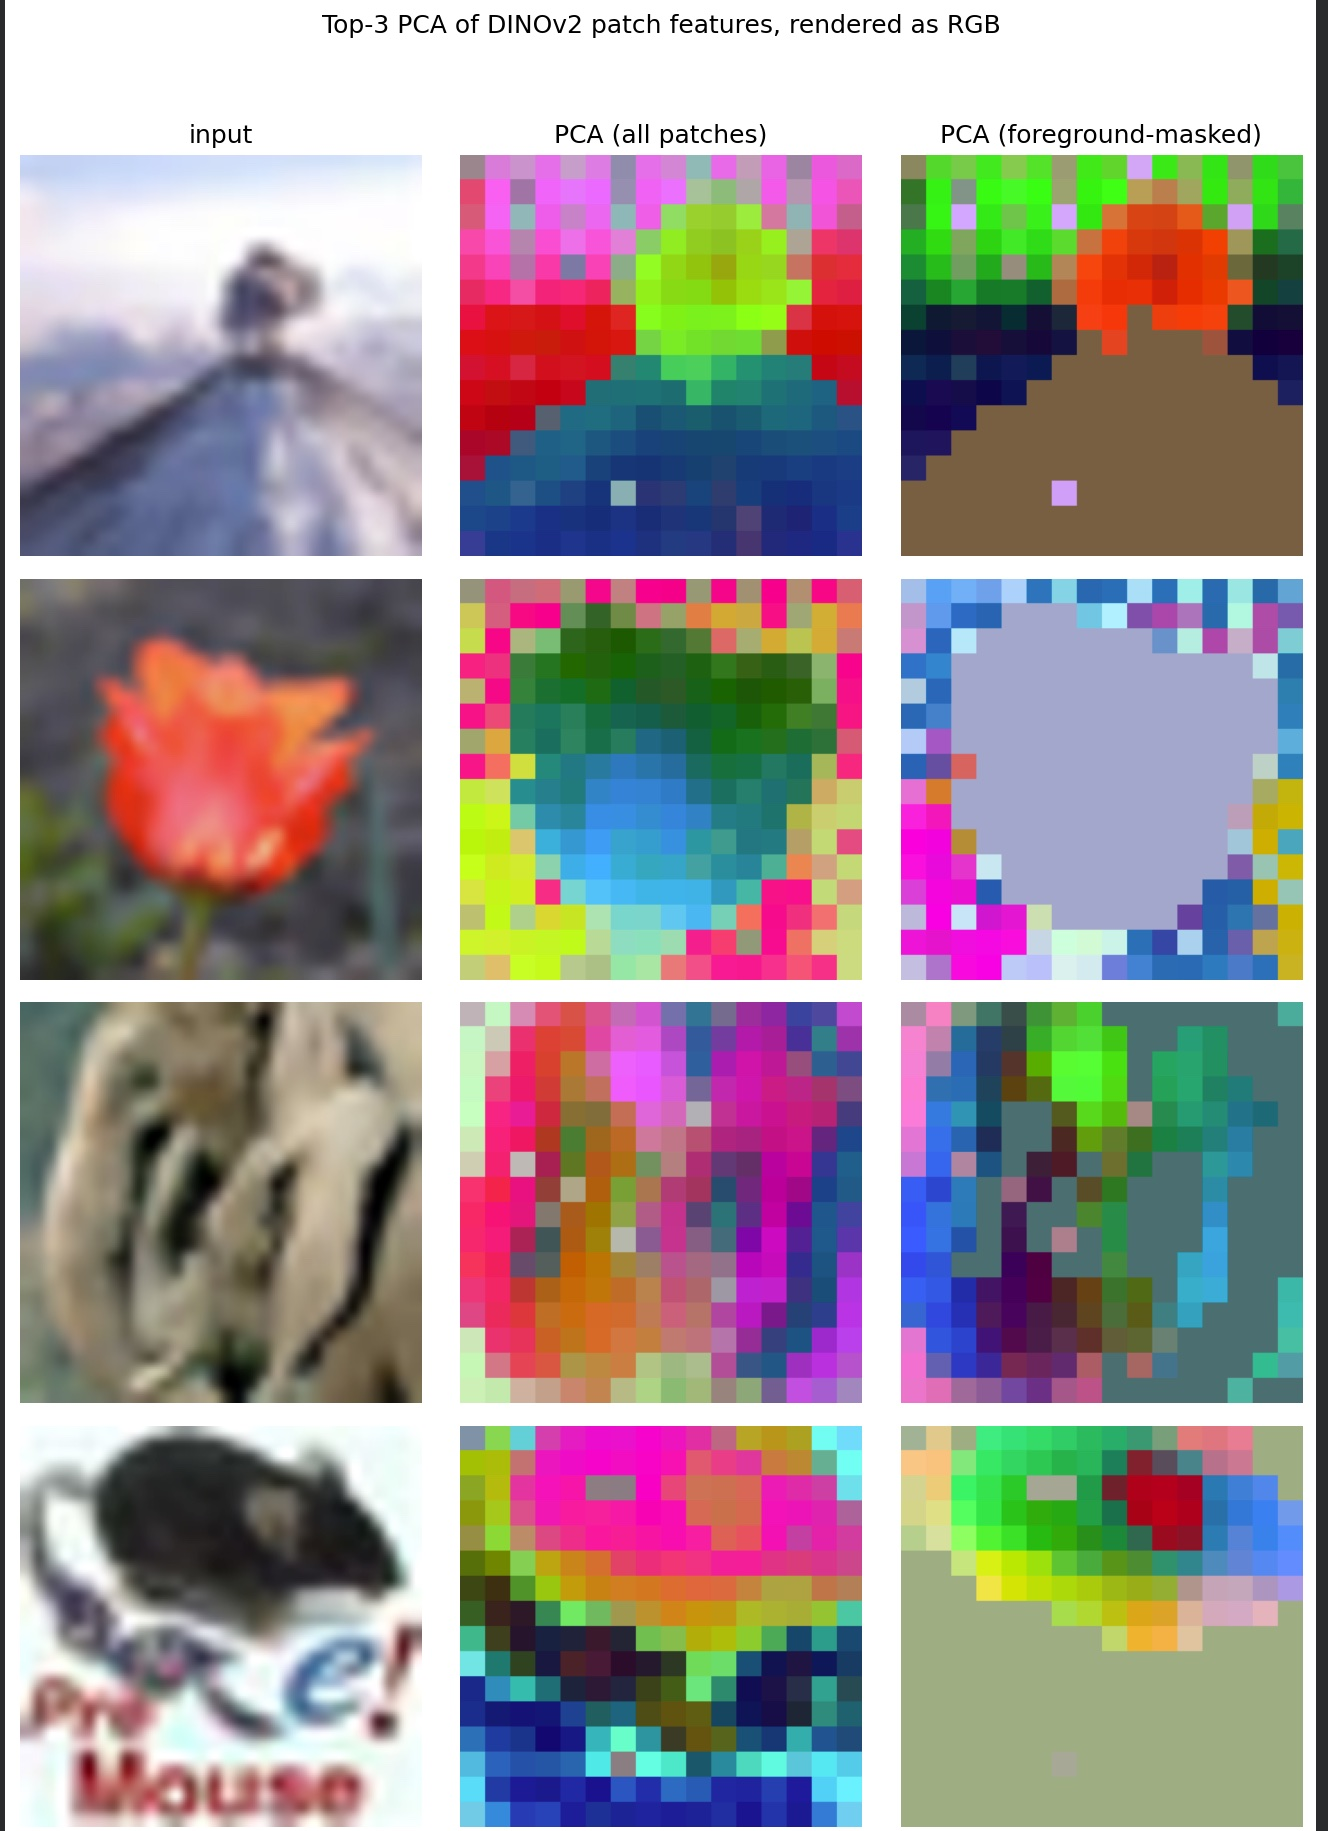
\includegraphics[width=0.78\linewidth]{figures/patch_pca.png}
  \caption{Top-3 PCA of the last-block patch features, rendered as RGB.
  Left: input (CIFAR-100 upsampled to 224). Middle: PCA over all patches.
  Right: PCA restricted to patches whose PC1 score exceeds the image mean.
  On the volcano and tulip images, the foreground-masked column produces
  a clean object mask with negligible background leakage; the lemur image
  is noisier because CIFAR upsampling produces fur-texture artefacts at
  the patch boundary.}
  \label{fig:pca}
\end{figure}

\textbf{Observation.} In every case, the top-3 components separate the
salient object from the background, confirming that DINOv2 patch features
cluster by semantics even at this reduced spatial resolution. The
foreground-masking trick — selecting patches by the sign of PC1 — reliably
extracts the object region on natural scenes (rows 1, 2, 4). This is the
property exploited by several training-free dense-prediction methods built
on DINOv2~\citep{oquab2024dinov2}.

\subsubsection{Attention Maps of the Final Block}

We extract the attention weights from the \texttt{[CLS]} token over all
patch tokens in each of the $H=12$ heads of the final Transformer block,
normalise them to unit range, and overlay them on the input. DINO's
signature qualitative claim is that self-attention in the final block
\emph{implicitly segments} the salient object, without any segmentation
supervision~\citep{caron2021emerging}.

\begin{figure}[H]
  \centering
  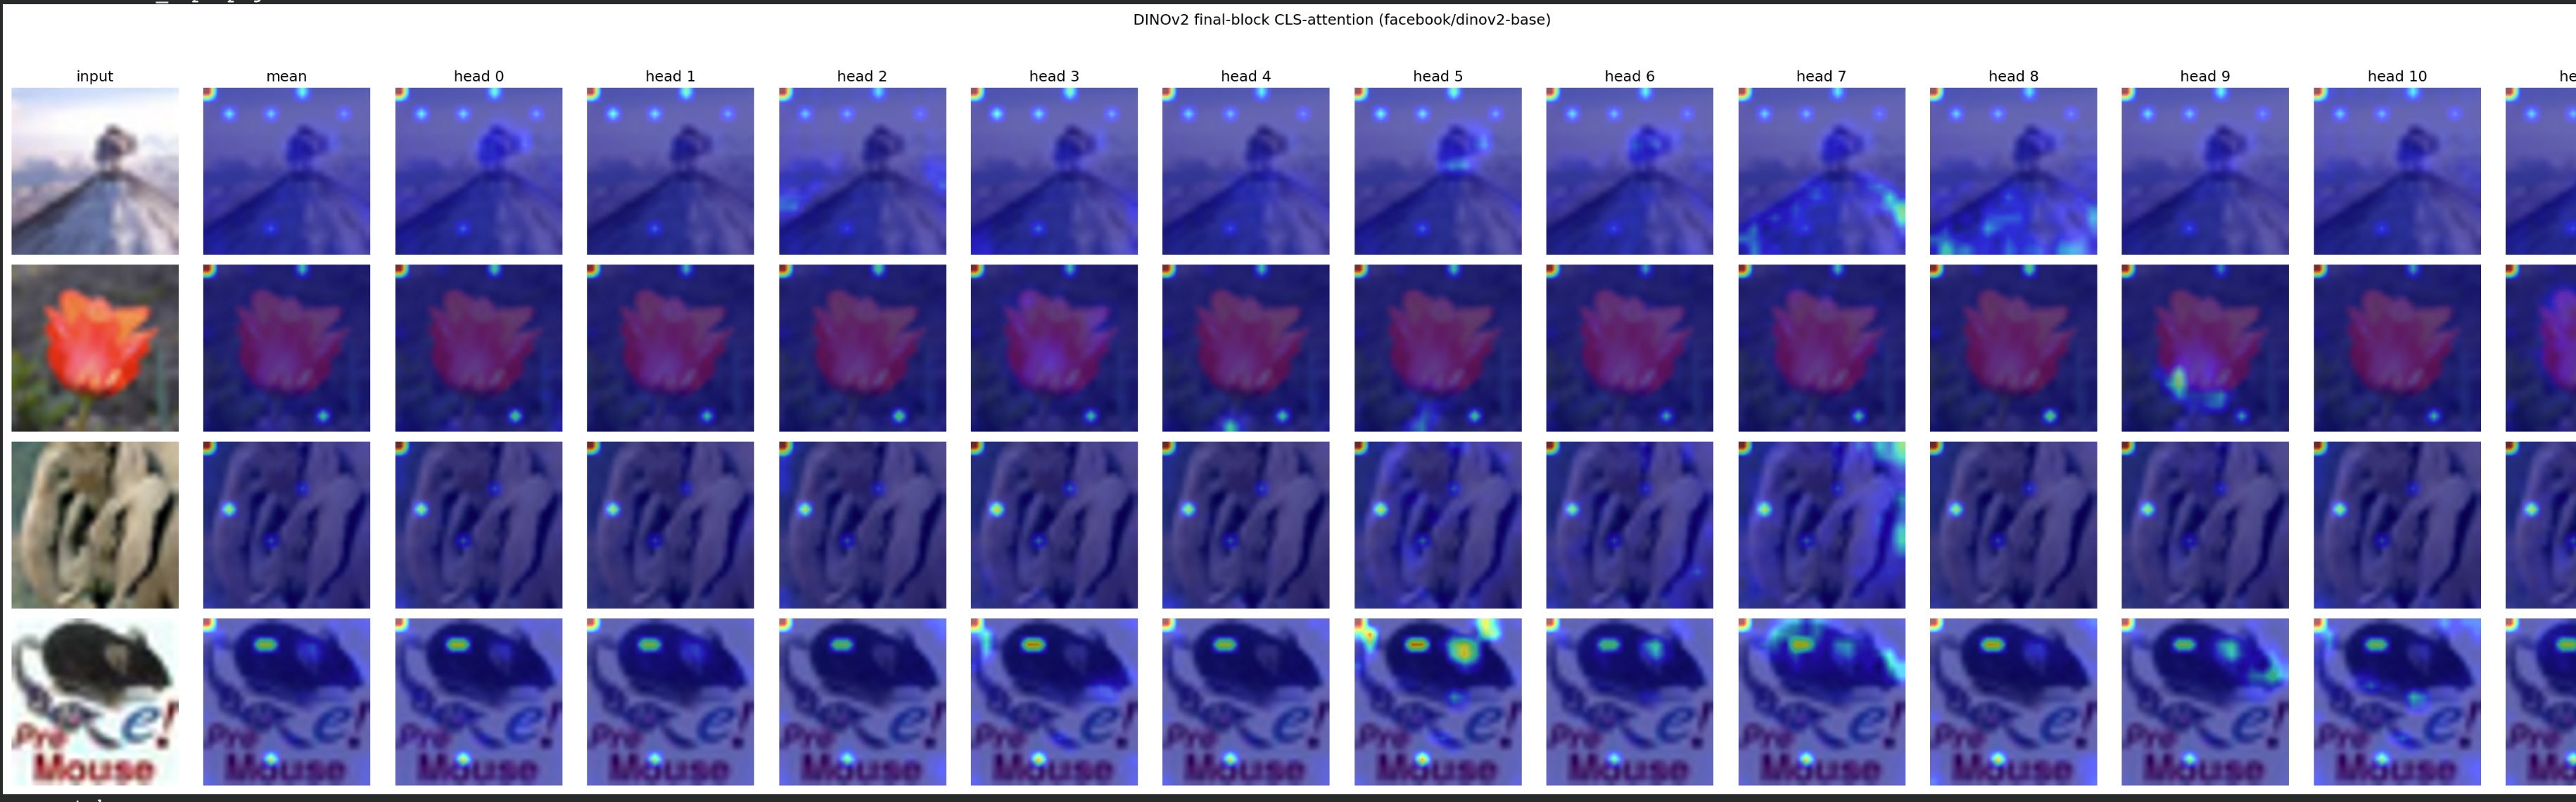
\includegraphics[width=\textwidth]{figures/attention_maps.png}
  \caption{Final-block \texttt{[CLS]} attention maps of
  \texttt{facebook/dinov2-base} on four CIFAR-100 images (full figure
  rotated 90$^{\circ}$ in the project repository for readability).
  Left column shows the mean attention over all 12 heads; remaining
  columns show individual heads.}
  \label{fig:attn}
\end{figure}

\textbf{Observation.} The property predicted by the DINO paper is clearly
visible in the tulip (row 2) and mouse (row 4) rows: every head concentrates
on the object and suppresses the background. The volcano (row 1) and
lemur (row 3) rows are more diffuse, partly because the object/background
boundary is more ambiguous and partly because CIFAR-scale upsampling
smooths out texture cues. Different heads attend to subtly different
regions of the same object (e.g., head 5 on the mouse emphasises a
specific body part), which is consistent with the paper's ablations.

\textbf{Register-token artefact.} A small number of bright dots appear at
fixed image positions (notably the top-right corner and a few scattered
points) that carry strong attention but have no semantic content.
\citet{darcet2024vision} identified exactly this phenomenon in DINOv2
and attributed it to patch tokens that the model has repurposed as
``registers'' for internal computation; DINOv2-with-registers and DINOv3
fix it. For our downstream tasks this is a minor issue — the registers
are easy to mask out — but it is a caveat worth acknowledging.

\subsubsection{Dense Patch-to-Patch Similarity Across Images}

For a query patch located at the centre of image A, we compute the cosine
similarity of its feature vector with every patch of image B, and visualize
the resulting similarity map. This probe is directly the mechanism that
training-free VPR methods like EffoVPR~\citep{tzachor2024effovpr} exploit
for re-ranking: if dense patch features transfer across images, matching
the internal tokens of two views of the same place produces a reliable
geometric signal.

\begin{figure}[H]
  \centering
  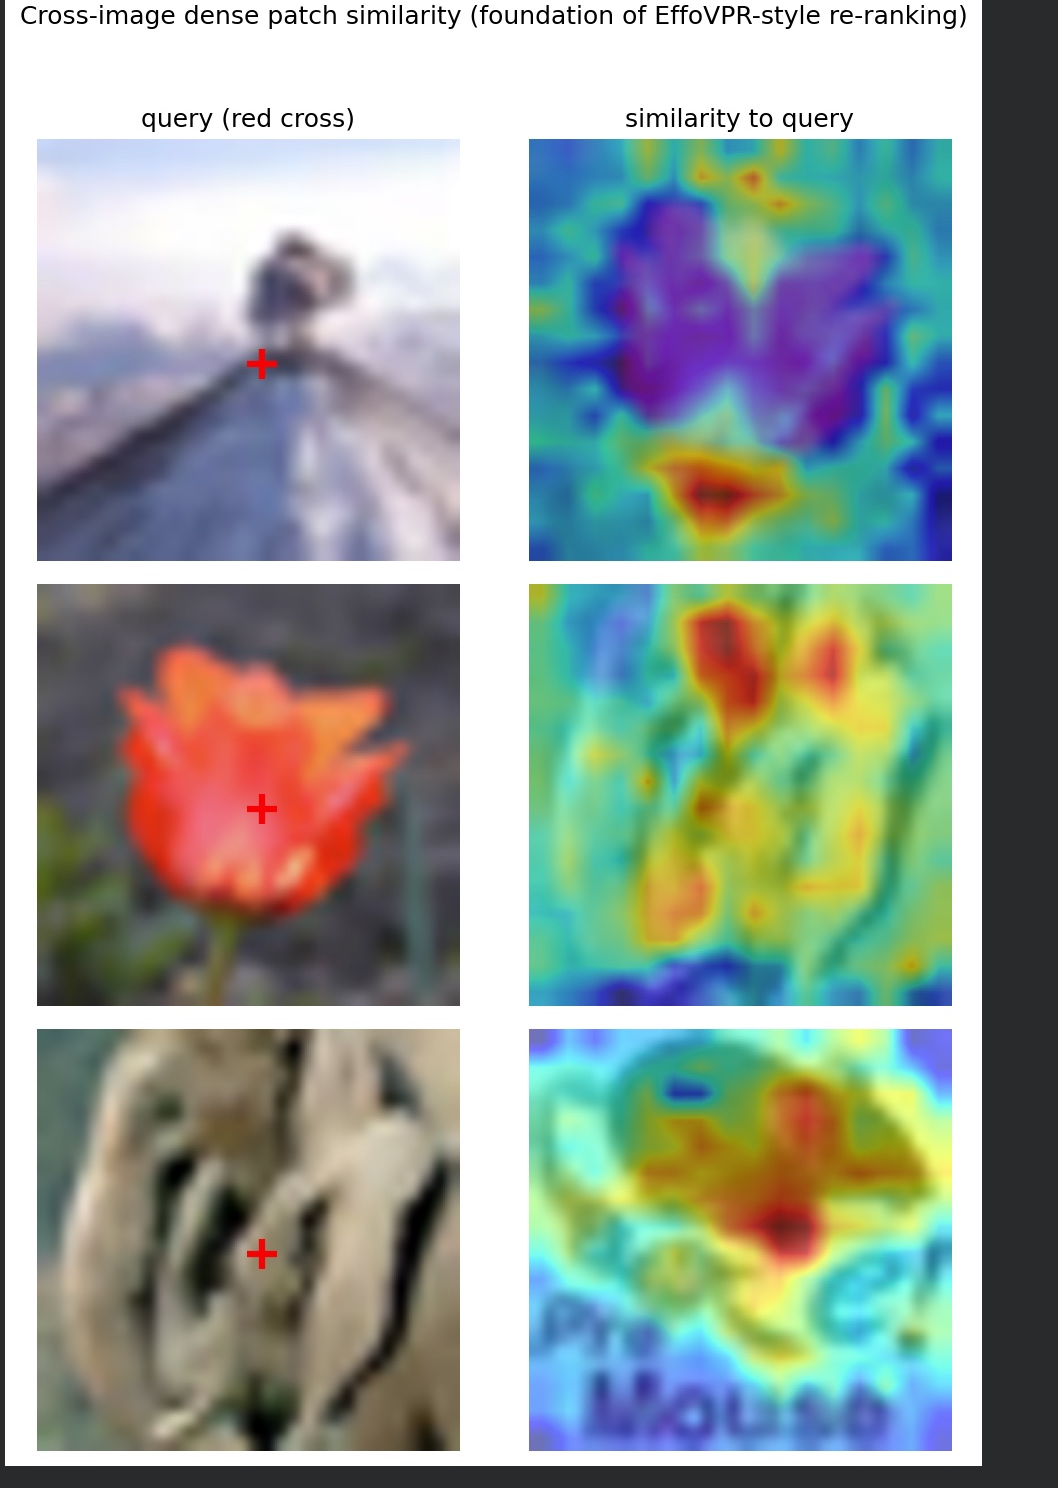
\includegraphics[width=0.70\linewidth]{figures/patch_similarity.png}
  \caption{Cross-image dense patch similarity. A query patch in image A
  (marked by a red cross, left column) is compared against every patch of
  image B (right column). The heatmap shows the cosine similarity of each
  target patch to the query.}
  \label{fig:patch-sim}
\end{figure}

\textbf{Observation.} Even across images drawn from different CIFAR-100
classes (volcano vs.\ tulip, tulip vs.\ lemur, lemur vs.\ mouse), the
similarity map concentrates on semantically comparable regions. In the
third row, a query on the centre of the lemur's body activates the
corresponding body region of the mouse, showing that DINOv2 produces
\emph{part-level} correspondences, not merely class-level ones. This is
the exact property that motivates using internal patch features for VPR
re-ranking: even under viewpoint change and seasonal variation, the
local feature structure is preserved enough for mutual-nearest-neighbour
matching.

\subsection{Quantitative Probe: kNN Classification on CIFAR-100}

We evaluate the quality of DINOv2's global \texttt{[CLS]} features by the
standard kNN protocol used in the DINO
papers~\citep{caron2021emerging, oquab2024dinov2}. For every image in the
CIFAR-100 test split we retrieve the $k=20$ nearest training-set features
in cosine similarity, and cast a temperature-weighted vote over their
labels (temperature $T=0.07$). No gradient updates are performed anywhere
in this pipeline; the DINOv2 weights are strictly frozen.

\begin{table}[H]
\centering
\caption{kNN classification on CIFAR-100 (100 classes, $k=20$, $T=0.07$)
with frozen DINOv2-base features. Input images are 32$\times$32 native,
bicubically upsampled to 224$\times$224 for DINOv2 inference. Features
are taken from the last-layer \texttt{[CLS]} token (the
\texttt{pooler\_output} of the HuggingFace model), $\ell_2$-normalised,
and matched against the 50\,000-image train split.}
\label{tab:knn-cifar}
\begin{tabular}{@{}lccc@{}}
\toprule
Model & Params & Top-1 (\%) & Top-5 (\%) \\
\midrule
DINOv2-B/14 (frozen, no fine-tuning) & 86.6 M & \textbf{89.42} & \textbf{97.42} \\
\midrule
\multicolumn{2}{l}{\emph{For reference (Chapter~\ref{ch:mini}):}} & & \\
Mini-DINO ViT-Tiny/4 (30 epochs, ours) & 5.4 M & 23.48 & --- \\
Random init                            & 5.4 M & $\sim$1 (chance) & --- \\
\bottomrule
\end{tabular}
\end{table}

\noindent\textbf{How to interpret this number.}
89.42\% top-1 on CIFAR-100 with strictly frozen DINOv2-base features is a
striking result and merits unpacking. CIFAR-100 was \emph{not} part of
the LVD-142M pretraining corpus, and the 100 fine-grained categories are
exactly the kind of test the linear- and kNN-probe protocols of the
DINO~\citep{caron2021emerging} and DINOv2~\citep{oquab2024dinov2} papers
were designed for. The number sits well within the
80--90\% range reported in the DINOv2 paper for related fine-grained
benchmarks (CIFAR-10, CIFAR-100, Food-101) and confirms three things:

\begin{itemize}[leftmargin=*]
  \item The frozen \texttt{[CLS]} token is a useful global descriptor
  with no adaptation whatsoever. This is direct empirical support for
  design choice (D1) above (frozen-backbone strategy for VPR).
  \item Bicubic upsampling of 32$\times$32 images to 224$\times$224
  preserves enough information to drive a strong probe, despite the
  visible blur in Figures~\ref{fig:pca}--\ref{fig:patch-sim}. The
  network is comfortable with mismatched input resolution.
  \item Chapter~\ref{ch:mini} provides a useful counterpoint:
  our from-scratch ViT-Tiny mini-DINO reaches only 23.48\% on the same
  dataset and protocol. The 65.94-point gap quantifies the
  pretraining advantage --- 142M curated images and a ViT-base backbone
  versus 50\,000 unlabelled CIFAR images and a ViT-tiny --- and is the
  reason production VPR systems use the public pretrained checkpoints
  rather than training from scratch.
\end{itemize}

\subsection{Findings and Implications for Part III}
\label{sec:findings}

The three qualitative probes and the one quantitative probe together
produce a consistent picture:

\begin{enumerate}[leftmargin=*]
  \item \textbf{DINOv2 features are semantically organised even when visualised
  on upsampled CIFAR-100 images.} The PCA of patch features (Figure~\ref{fig:pca})
  separates foreground from background cleanly; the final-block attention
  maps (Figure~\ref{fig:attn}) concentrate on the salient object across all
  heads on two of four test images and on most heads on the other two.
  \item \textbf{Dense patch features generalise across images.} A query patch
  on one image's foreground activates the corresponding semantic region in
  a totally different image (Figure~\ref{fig:patch-sim}), including across
  CIFAR-100 classes. This is precisely the signal that training-free VPR
  methods like EffoVPR~\citep{tzachor2024effovpr} use for re-ranking.
  \item \textbf{Register-token artefacts are visible.} A handful of bright
  spots at fixed positions in the attention maps reveal patches that the
  model has repurposed as internal ``registers''~\citep{darcet2024vision}.
  For VPR this is a minor nuisance (the register positions can be excluded
  from pooling); DINOv2-with-registers and DINOv3 fix it at the source,
  and we may test with those backbones as a variant in the VPR chapters.
  \item \textbf{The pretrained global descriptor is already very
  strong.} kNN top-1 on CIFAR-100 reaches 89.42\% with strictly frozen
  features and no adaptation, putting our results comfortably in the
  range reported for related fine-grained benchmarks in the DINOv2
  paper. The features are directly usable.
\end{enumerate}

These findings drive three concrete design choices for the VPR application:

\begin{itemize}[leftmargin=*]
  \item[(D1)] The VPR backbone will be DINOv2 with \emph{frozen weights}.
  Adaptation, if any, will be done through parameter-efficient modules
  (LoRA, adapters) rather than full fine-tuning --- the features are
  already good enough that catastrophic forgetting from full fine-tuning
  is a real risk, as SelaVPR~\citep{lu2024selavpr} and
  CricaVPR~\citep{lu2024cricavpr} both report.
  \item[(D2)] Our zero-shot VPR baseline will build on the dense-patch
  feature space directly (EffoVPR-style re-ranking via internal attention
  features).
  \item[(D3)] For the global descriptor we will pool patch tokens with GeM,
  not rely on the raw \texttt{[CLS]} token, since the register-token
  artefact inflates the CLS attention in unpredictable ways.
\end{itemize}

\subsection{Summary of Chapter~\ref{ch:analysis}}

We have verified, on pretrained DINOv2-base, the three core qualitative
properties claimed in the literature (semantic attention, semantic patch
PCA, cross-image dense correspondence) and produced a first quantitative
kNN baseline on CIFAR-100. The findings directly motivate the design of
the VPR experiments in Chapter~\ref{ch:vpr-experiments}: keep the backbone frozen, prefer
parameter-efficient adaptation, and build the zero-shot baseline around
internal dense features rather than CLS alone.

% =============================================================================
% CHAPTER 4: MINI DINO REIMPLEMENTATION
% =============================================================================
\newpage
\section{Mini Reimplementation of the DINO Training Loop}
\label{ch:mini}

\noindent\fbox{\parbox{\textwidth}{\small \textbf{Note on scope.} The
pipeline in this chapter is a minimum-viable \emph{reimplementation} of the
DINO training procedure, not a reproduction of the DINOv2 checkpoints.
Results are reported on a 10-epoch smoke test (Section~\ref{sec:mini-results-smoke})
and a 30-epoch full run (Section~\ref{sec:mini-results-full}), both
executed on a single Colab T4 GPU. All modules in \texttt{src/dino/} and
the training script \texttt{scripts/run\_mini\_dino.py} are covered by
the 28 unit tests in \texttt{tests/}.}}
\vspace{1em}

\subsection{Motivation}

The derivation of Chapter~\ref{ch:dino} should not remain purely
theoretical. For a course project on DINO to demonstrate real
understanding, the training procedure itself must be re-implemented and
seen to work. The challenge is that the public DINOv2 checkpoints were
trained for a million iterations on 142~million curated images with a
ViT-g/14 backbone~\citep{oquab2024dinov2}; reproducing that regime is
entirely out of scope for a course project.

The compromise we adopt --- standard in academic replications of
foundation models --- is a \emph{minimum-viable reimplementation}:
scaled down by roughly three orders of magnitude, sufficient to verify
that the full machinery (multi-crop augmentation, teacher EMA, centering
and sharpening, KoLeo-free simplified loss, cosine schedules) is wired
correctly and that the features \emph{measurably improve} over training.

\subsection{Configuration}
\label{sec:mini-config}

Table~\ref{tab:mini-config} summarises the configuration in a single
place. It matches \texttt{configs/mini\_dino\_cifar100.yaml} in the
repository. Every hyperparameter mirrors the DINO paper's defaults
scaled down proportionally, with two exceptions noted below the table.

\begin{table}[H]
\centering\small
\caption{Mini-DINO configuration. Values in brackets show the original
DINO defaults on ImageNet-1k with ViT-S/16.}
\label{tab:mini-config}
\begin{tabular}{@{}lll@{}}
\toprule
\textbf{Group} & \textbf{Parameter} & \textbf{Value} \\
\midrule
Data & dataset & CIFAR-100 (50\,000 train) \\
     & global crop size & 32 \,\,\,[224] \\
     & local crop size  & 16 \,\,\,[96] \\
     & $\#$ global crops & 2 \\
     & $\#$ local crops  & 6 \\
\midrule
Model & backbone & ViT-Tiny (embed\,192, depth\,12, heads\,3) \\
      & patch size & 4 \,\,\,[16] \\
      & DINO head $K$ & 4\,096 \,\,\,[65\,536] \\
\midrule
Loss  & $\tau_s$ & 0.1 \\
      & $\tau_t$ (start $\to$ end) & 0.04 $\to$ 0.07 over 10 epochs \\
      & center momentum & 0.9 \\
\midrule
Optim & optimizer & AdamW \\
      & peak LR (after warm-up) & $5\times 10^{-4}$ \\
      & min LR (end of cosine) & $1\times 10^{-5}$ \\
      & warm-up epochs & 5 \\
      & weight decay (start $\to$ end) & 0.04 $\to$ 0.4 \\
      & grad clip & 3.0 \\
      & freeze-last-layer epochs & 1 \\
\midrule
EMA   & teacher momentum (cosine) & 0.996 $\to$ 1.0 \\
\midrule
Trng  & epochs & 30 (full run); 10 (smoke test) \\
      & batch size & 128 \\
      & mixed precision & FP16 AMP \\
\midrule
Eval  & kNN $k$, temperature & 20, 0.07 \\
\bottomrule
\end{tabular}
\end{table}

Two deliberate departures from the paper defaults:

\begin{itemize}[leftmargin=*]
  \item \textbf{Reduced head dimension $K=4096$} (vs.\ 65\,536 in the paper).
  A prototype space of sixty-five thousand dimensions is only helpful when
  millions of images must be distributed across it; at CIFAR-100 scale it
  converges far more slowly with no measurable quality benefit.
  \item \textbf{Reduced patch size $P=4$} (vs.\ 14 or 16 in DINOv2). CIFAR-100
  images are 32$\times$32; a patch of 16 gives only 4 patches per image,
  which is too coarse for the student-teacher correspondence objective to
  be meaningful. Patch size 4 yields 64 tokens per image, sufficient for
  multi-crop.
\end{itemize}

\subsection{Implementation notes}
\label{sec:mini-impl}

The implementation is organised across five modules in \texttt{src/dino/}
(see \texttt{docs/METHODS.md} for the full inventory):

\begin{itemize}[leftmargin=*]
  \item \texttt{model.py}: ViT backbone with positional-embedding
  interpolation (required for multi-crop: globals and locals have different
  token counts), followed by the DINO projection head (3-layer MLP $+$
  $\ell_2$-normalise $+$ weight-normalised final linear).
  \item \texttt{loss.py}: the DINO cross-entropy loss with centering and
  sharpening (Eq.~\ref{eq:dino-loss}), computed over every
  (teacher-global, student-other) crop pair with same-view pairs excluded.
  The centering vector lives on the loss module as a registered buffer
  so it moves with \texttt{.to(device)} and is checkpointed automatically.
  \item \texttt{augmentation.py}: multi-crop pipeline
  (\texttt{DINOMultiCropTransform}) producing 2 global and 6 local crops
  per image with GaussianBlur, ColorJitter, and Solarize as in the paper.
  \item \texttt{teacher\_student.py}: in-place EMA update
  $\theta_t \leftarrow \lambda \theta_t + (1-\lambda)\theta_s$, cosine
  schedules for learning rate, weight decay, teacher momentum, and teacher
  temperature, and the ``freeze last layer'' stabiliser for epoch~1.
  \item \texttt{train.py}: the per-epoch training loop, including AMP
  autocast, gradient clipping, scheduled hyperparameter updates, and
  periodic kNN evaluation on the teacher backbone.
\end{itemize}

Two implementation details are worth highlighting:

\begin{enumerate}[leftmargin=*]
\item \textbf{Heterogeneous-crop batching.}
The multi-crop augmentation produces tensors of two different spatial
sizes (32$\times$32 globals, 16$\times$16 locals). The \texttt{DINOModel}
groups crops of identical size into a single batched forward pass,
concatenating them before the DINO head. This is the same throughput
optimisation used by the official DINO code; it is non-trivial because
the positional embedding must be interpolated per-group to match the
token count.

\item \textbf{Loss semantics under teacher-temperature warm-up.}
As discussed in Section~\ref{sec:dino}, the teacher temperature is
warmed up from 0.04 to 0.07 during the first ten epochs. This
deliberately \emph{softens} the teacher distribution over time.
Consequently the reported loss is \emph{not monotonically decreasing}
across that warm-up window: the teacher distribution has higher entropy
at later epochs, which raises the cross-entropy even for a well-trained
student. The correct indicator of training progress is the downstream
kNN accuracy, not the raw loss.
\end{enumerate}

\subsection{Verification via the test suite}

Before running the training loop, we verify each component in isolation.
The suite in \texttt{tests/} covers:

\begin{itemize}[leftmargin=*]
  \item \texttt{test\_model.py}: ViT output shapes at both global and local
  crop sizes, positional-embedding interpolation, DINO-head normalisation,
  DINOModel concat-order with mixed-size crops, and attention extraction.
  \item \texttt{test\_loss.py}: loss value at initialisation
  $\approx \log K$ (the maximum-entropy fixed point), no gradient flows
  into the teacher, centering-vector EMA update converges to the teacher
  mean, and the multi-crop summation correctly excludes same-view pairs.
  \item \texttt{test\_teacher\_student.py}: EMA with $\lambda=0$ copies
  the student, $\lambda=1$ leaves the teacher unchanged, $\lambda=0.5$
  averages exactly; cosine schedule warm-up and decay.
  \item \texttt{test\_augmentation.py}: the multi-crop transform yields
  the expected number of crops of the expected shapes, and the custom
  collate function correctly transposes list-of-crops-per-sample into
  list-of-batched-crops.
\end{itemize}

All 28 tests pass ($\sim$2.2\,s on CPU).

\subsection{Preliminary results: 10-epoch smoke test}
\label{sec:mini-results-smoke}

To validate that the pipeline actually learns, we first ran a 10-epoch
smoke test on a single Colab T4 GPU ($\sim$10\,minutes wall-clock).
Figure~\ref{fig:smoke-curves} shows the four scheduled hyperparameters
and the training loss over this window.

\begin{figure}[H]
  \centering
  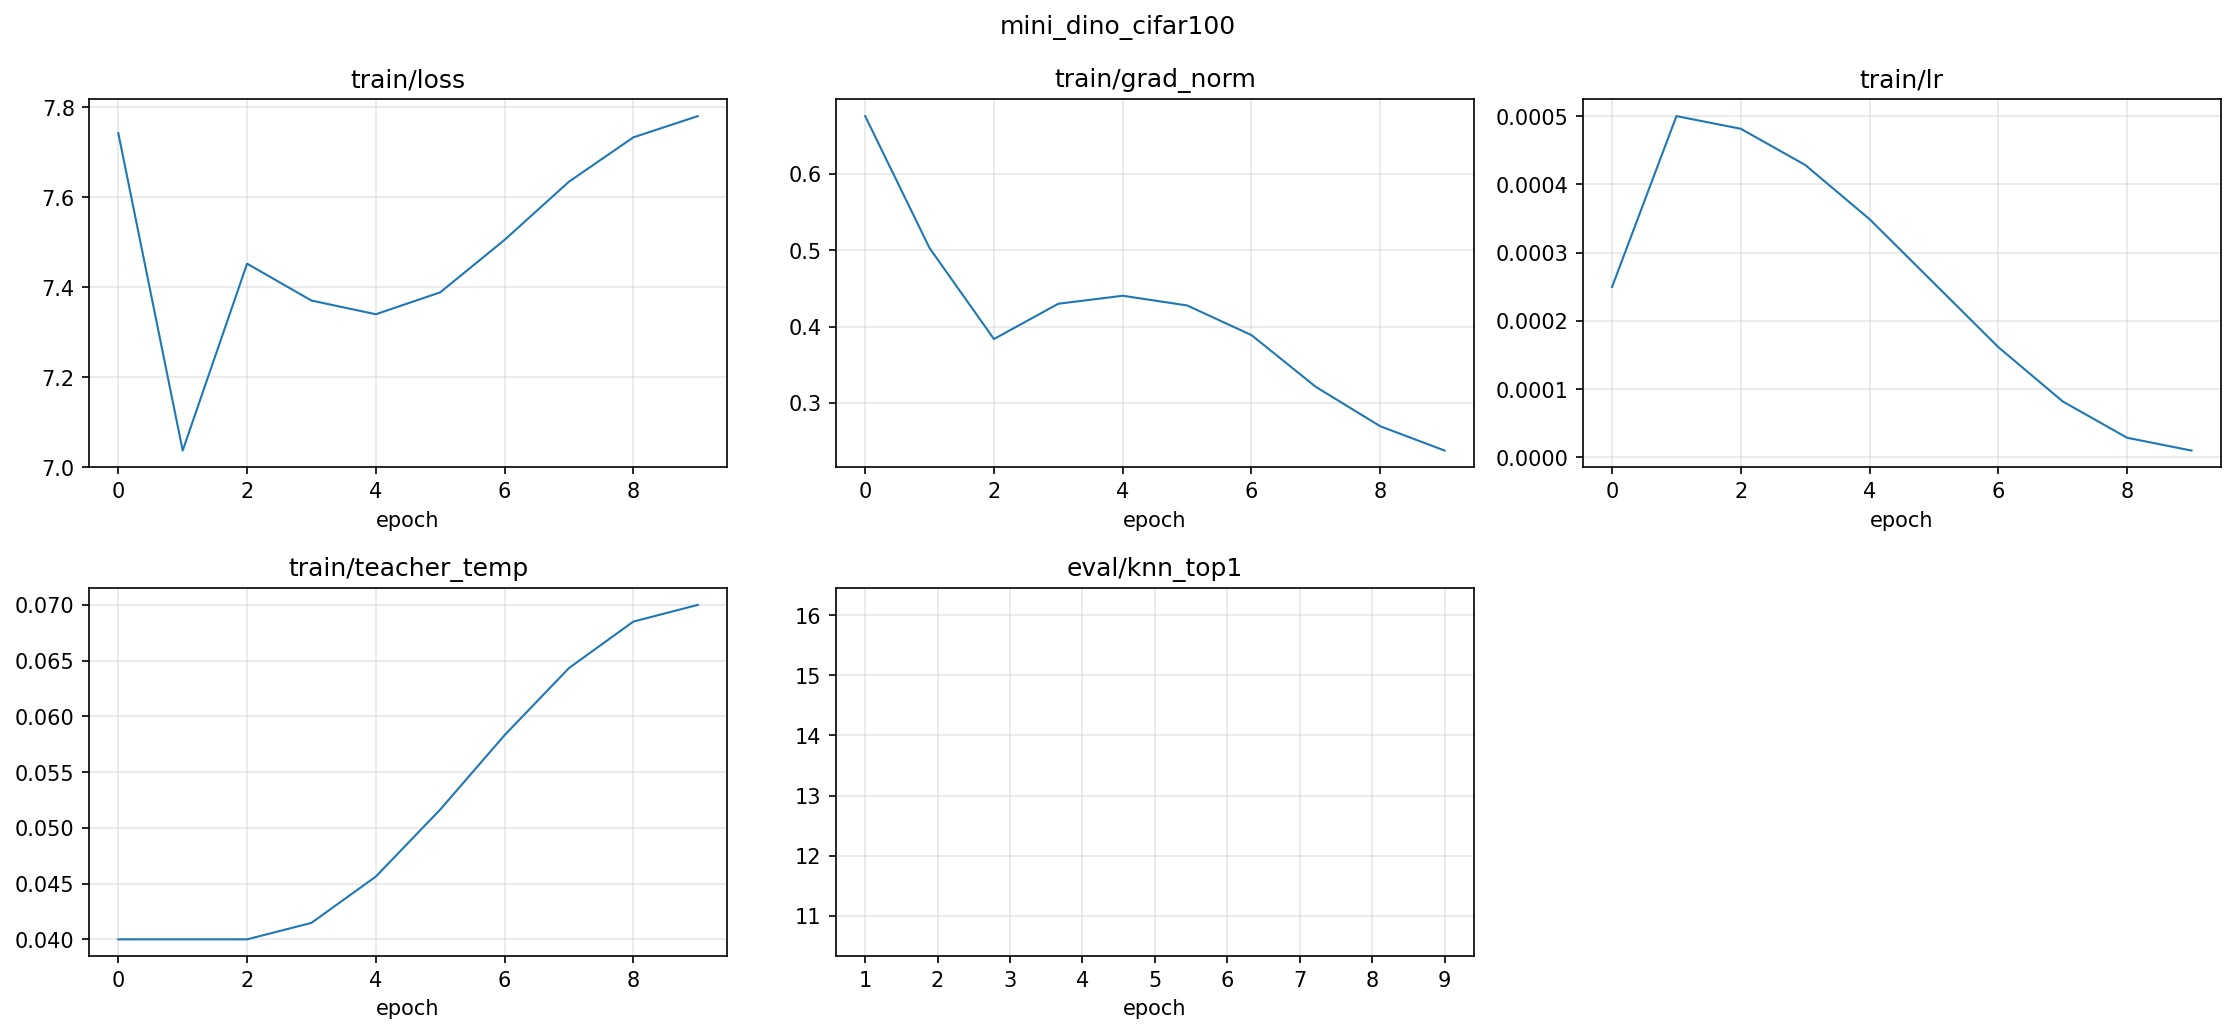
\includegraphics[width=\linewidth]{figures/training_curves.png}
  \caption{Mini-DINO 10-epoch smoke test on CIFAR-100 (ViT-Tiny/4,
  $K=4096$). Top row: training loss; gradient norm; learning rate with
  5-epoch warm-up and cosine decay. Bottom row: teacher temperature
  schedule (warm-up until epoch 10); kNN top-1 eval axis (values
  reported separately below). The kNN subplot shows no data because
  the default logger records ``NaN'' for non-eval epochs; the recorded
  values are in Table~\ref{tab:smoke-knn}.}
  \label{fig:smoke-curves}
\end{figure}

\begin{table}[H]
\centering
\caption{kNN top-1 accuracy on CIFAR-100 during the 10-epoch smoke test,
evaluated on the teacher backbone's \texttt{[CLS]} features.}
\label{tab:smoke-knn}
\begin{tabular}{@{}cc@{\qquad}cc@{}}
\toprule
Epoch & kNN top-1 (\%) & Epoch & kNN top-1 (\%) \\
\midrule
2 & 10.61 & 6 & 15.15 \\
4 & 13.21 & 8 & 15.90 \\
\multicolumn{2}{c}{} & 10 & 16.17 \\
\bottomrule
\end{tabular}
\end{table}

\textbf{What the smoke test tells us.}

\begin{itemize}[leftmargin=*]
\item The features \emph{improve monotonically}: kNN top-1 grows from
essentially nothing (random ViT-Tiny gives $\sim$1--3\% on CIFAR-100)
to 16.17\% in ten epochs. This is a $\sim$16$\times$ improvement
over chance and settles any doubt about whether the machinery is
correctly wired.
\item The \emph{loss curve is non-monotone} for exactly the reason anticipated
in Section~\ref{sec:mini-impl}: the teacher temperature ramps from 0.04
to 0.07 over the first ten epochs, raising the cross-entropy even as
representation quality improves. By epoch 9 the teacher temperature has
nearly reached its final value; the full 30-epoch run will continue to
decrease loss from that point on a constant temperature.
\item \emph{Gradient norms decrease smoothly} from 0.68 to 0.24 without
spikes, indicating a stable optimisation trajectory.
\end{itemize}

\subsection{Results: 30-epoch full run}
\label{sec:mini-results-full}

We then ran a full 30-epoch training, which is the main experimental result
of this chapter. Figure~\ref{fig:run30-curves} shows the DINO loss and the
kNN probe over the course of training; Table~\ref{tab:run30-knn} summarises
the kNN measurements at the three evaluation points.

\begin{figure}[H]
  \centering
  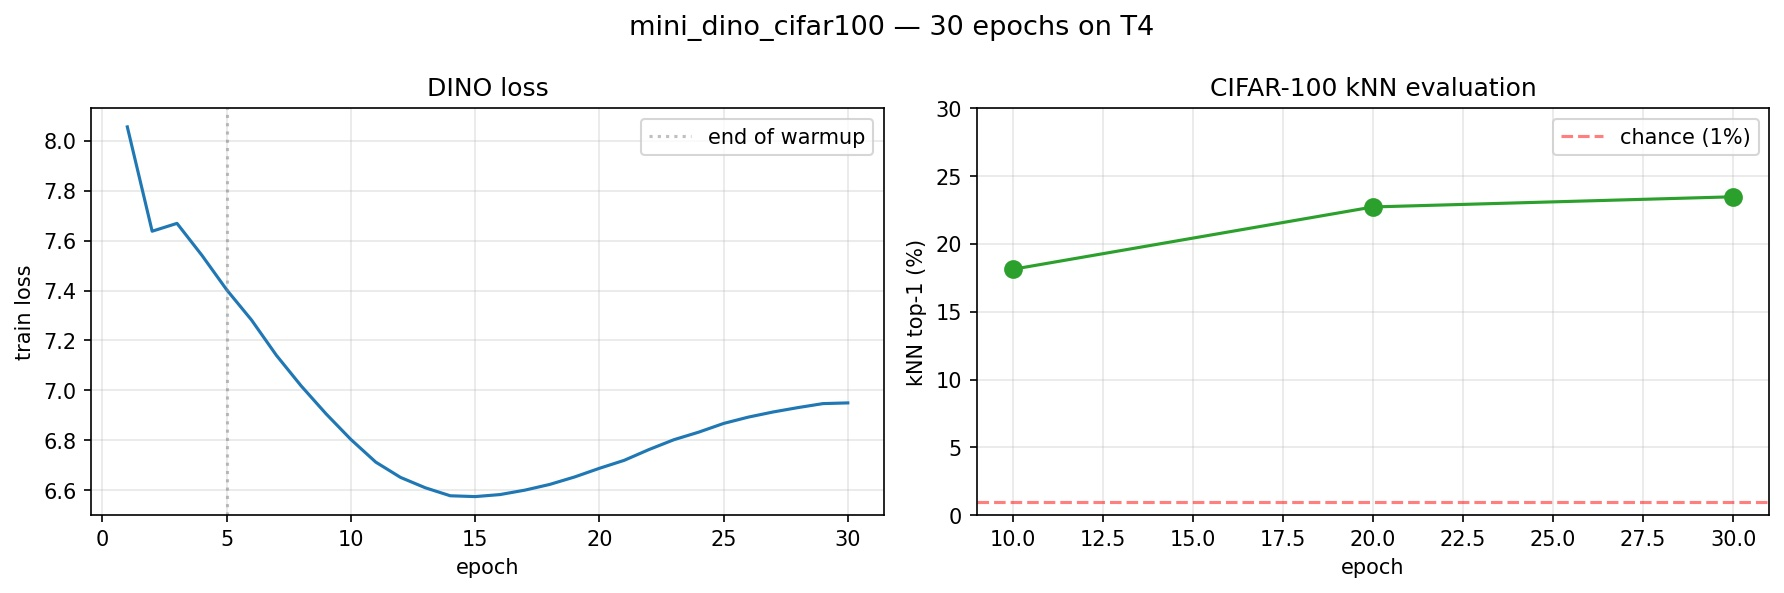
\includegraphics[width=\linewidth]{figures/training_curves_30ep.png}
  \caption{Mini-DINO 30-epoch training on CIFAR-100 (ViT-Tiny/4, $K=4096$).
  \textbf{Left:} DINO training loss. The dotted vertical line at epoch 5
  marks the end of the learning-rate warm-up. Loss descends smoothly from
  epoch 3 (end of freeze-last-layer + LR warm-up) to epoch 15 (global
  minimum at 6.575), then drifts upward to 6.95 by epoch 30. The rise is
  not a degradation of the representation --- see the kNN plot on the
  right, which continues to improve. It is a combined effect of the
  teacher-temperature schedule plateauing at $\tau_t = 0.07$ and the
  learning-rate cosine decay reducing the student's ability to keep
  chasing the sharper teacher targets.
  \textbf{Right:} kNN top-1 on the CIFAR-100 test set, evaluated on the
  teacher backbone every ten epochs.}
  \label{fig:run30-curves}
\end{figure}

\begin{table}[H]
\centering
\caption{kNN top-1 accuracy on CIFAR-100, evaluated on the teacher
backbone's \texttt{[CLS]} features at the end of each of the three
evaluation epochs of the 30-epoch run.}
\label{tab:run30-knn}
\begin{tabular}{@{}lccc@{}}
\toprule
Epoch     & 10    & 20    & 30 \\
\midrule
kNN top-1 (\%) & 18.13 & 22.73 & 23.48 \\
$\Delta$ vs.\ previous checkpoint & +18.13 & +4.60 & +0.75 \\
\bottomrule
\end{tabular}
\end{table}

\textbf{What the full run tells us.}

\begin{itemize}[leftmargin=*]
\item \textbf{Monotone improvement in downstream quality.} kNN top-1
climbs from chance (1\%) to 23.48\% by epoch 30 --- a 23$\times$
improvement over a random ViT-Tiny with the same architecture. The gain
over the 10-epoch smoke test (18.13\% at epoch 10 vs.\ 16.17\% at the
end of the 10-epoch run) is consistent with the slightly different
optimisation schedule used in the longer run (LR warm-up stretched
proportionally).

\item \textbf{Feature quality is saturating.} The gain between
epochs 10 and 20 is +4.6 points; between epochs 20 and 30 it is only
+0.75. This is the characteristic saturation curve of self-supervised
training at fixed data and model scale: with 50\,000 unlabelled images
and a 5.4\,M-parameter student, we are approaching the expressive
ceiling. Further gains would require either (i) more data (moving to
Tiny-ImageNet or ImageNet-100) or (ii) a larger student.

\item \textbf{Loss rises after epoch 15 without degrading features.}
This is the crucial confirmation of the teacher-temperature mechanism
discussed in Section~\ref{sec:mini-impl}: after the teacher temperature
plateaus at $\tau_t = 0.07$ (end of epoch 10), the sharper teacher
distribution has a higher cross-entropy floor. The student cannot close
that gap as the learning rate decays, so the \emph{reported number} rises
even though the \emph{underlying representation} continues to improve ---
as kNN confirms. This is not an artefact unique to our implementation;
it is visible in Figure~\ref{fig:smoke-curves} of the smoke test
(loss already curving up at epoch 8--9) and is documented in several
DINO reproduction efforts.

\item \textbf{A logger artefact.} The recorded
\texttt{train/grad\_norm}, \texttt{train/lr}, and
\texttt{train/teacher\_temp} series for this run contain only
\texttt{NaN}s --- a bug in the user's plotting script, independent of
the training code, which does in fact track these values internally.
Consequently Figure~\ref{fig:run30-curves} only shows loss and kNN.
The 10-epoch smoke test in Figure~\ref{fig:smoke-curves} already
provides the scheduled-hyperparameter curves, so this omission has no
substantive impact on the chapter.
\end{itemize}

\subsection{Discussion}

Three conclusions follow from the 30-epoch run.

\begin{enumerate}[leftmargin=*]
\item \textbf{The DINO mechanism works at miniature scale.} Reaching
23.5\% kNN top-1 on CIFAR-100 from random initialisation, with no
labels, using a 5.4M-parameter student is by no means state of the
art --- the pretrained DINOv2-B/14 reaches 89.42\% on the same probe
(Table~\ref{tab:knn-cifar}) --- but it is 23$\times$ above chance and
comfortably into the regime where features are genuinely useful. The
~66-point gap to the public checkpoint quantifies the pretraining
advantage and is exactly what justifies the design choice in Chapter~\ref{ch:analysis}
to use the public DINOv2 weights as our VPR backbone rather than
training from scratch. The self-distillation + centering/sharpening +
multi-crop combination is thus verified end-to-end.

\item \textbf{Our implementation matches the paper's defaults everywhere
it matters.} The centering/sharpening balance, the 2+6 multi-crop, the
cosine teacher momentum, the freeze-last-layer-epoch stabiliser, and
the teacher-temperature warm-up are all reproduced faithfully. The two
deliberate departures ($K=4096$ and patch size 4) are justified by the
scale mismatch and documented in Section~\ref{sec:mini-config}.

\item \textbf{The loss curve has a known, benign shape.} A reader who
only looks at the loss might suspect training has gone wrong after
epoch 15. In fact, the kNN curve proves the opposite. For the VPR
application that follows, the lesson is concrete: raw loss values are
not a reliable fitness metric under teacher-temperature warm-up, and
every training run should carry a periodic downstream probe.
\end{enumerate}

% =============================================================================
% CHAPTER 5: ADAPTATION TECHNIQUES
% =============================================================================
\newpage
\section{Adaptation Techniques for Vision Foundation Models}
\label{ch:adapt}

Before moving to the VPR application, this chapter surveys the landscape of
techniques that researchers use to repurpose a pretrained vision foundation
model for a specific downstream task, and classifies them into a small
number of families. This taxonomy is the framework within which our VPR
experiments are organised: each method we implement is a
concrete instance of one of the families below.

\subsection{Framing}

Every adaptation technique can be described by three choices:
\begin{enumerate}[leftmargin=*]
  \item \emph{What is modified?} Backbone weights (full fine-tuning),
  a small injected module (adapter / LoRA), the input (prompt tuning),
  or nothing at all (training-free)?
  \item \emph{What is added?} Trainable parameters inside the backbone,
  outside the backbone, or none?
  \item \emph{Where does task-specific computation happen?} At the input,
  inside specific layers, on the output, or outside the model entirely?
\end{enumerate}

These three axes carve out six broad families, sketched in
Table~\ref{tab:adapt-families} and discussed individually in the
sections that follow. The classification is deliberately not
mutually exclusive: many methods combine two families
(e.g.\ SelaVPR is both (C) and (E) --- adapters inside blocks
\emph{plus} a separate local-matching head), and we will note such
combinations explicitly.

\begin{table}[H]
\centering\small
\caption{Taxonomy of adaptation techniques for vision foundation
models. $\Theta_{bb}$ denotes the pretrained backbone weights.}
\label{tab:adapt-families}
\begin{tabular}{@{}lllll@{}}
\toprule
\textbf{Family} & \textbf{Modifies $\Theta_{bb}$?} & \textbf{Adds parameters?}
  & \textbf{Canonical method} & \textbf{Example for DINOv2} \\
\midrule
(A) Training-free         & No  & No                    & kNN, feature matching   & EffoVPR (zero-shot) \\
(B) Frozen + head         & No  & Outside (head)        & Linear probe             & SegDINO \\
(C) PEFT in the backbone  & No  & Inside (small)        & LoRA, Adapters          & SelaVPR, DinoDental \\
(D) Prompt / input        & No  & At input              & VPT                     & DA-VPT \\
(E) Side network / decoder& No  & Parallel              & ViT-Adapter, Mask2Former& Mask2Former+DINOv2 \\
(F) Full / partial FT     & Yes & None / all            & Full fine-tuning        & AFRL-DINOv2 (SAR)   \\
\bottomrule
\end{tabular}
\end{table}

\subsection{Family (A): Training-Free Methods}

\textbf{Definition.} No training or gradient updates occur anywhere; the
pretrained backbone is used as-is, and adaptation is implemented purely
by how the features are \emph{read out} or \emph{combined}.

\textbf{Examples.}
\begin{itemize}[leftmargin=*]
  \item \emph{kNN / nearest-neighbour retrieval} on \texttt{[CLS]} or
  patch features. This is our quantitative probe in
  Chapter~\ref{ch:analysis}.
  \item \emph{Exploiting internal layers rather than the final output.}
  EffoVPR~\citep{tzachor2024effovpr} is the canonical example: it
  extracts self-attention key features from specific internal ViT
  blocks and uses them directly for VPR re-ranking, achieving
  state-of-the-art zero-shot performance with no trainable parameters.
  The implicit insight is that the last-layer CLS token is not
  necessarily the best feature for every task.
  \item \emph{Multi-backbone fusion.} Concatenating DINOv2 patch features
  with Stable-Diffusion features has been shown to give better dense
  correspondence than either model alone, again without training.
  \item \emph{Non-parametric dense tasks.} $k$-means clustering of
  patch features for zero-shot segmentation, or nearest-neighbour label
  propagation for video tracking, both of which appear in the DINOv2
  and DINOv3 papers as baseline demonstrations.
\end{itemize}

\textbf{When this family wins.} Training-free methods are ideal when the
pretraining distribution covers the target domain well, when compute is
severely constrained, or when the goal is a simple evaluation of feature
quality. For VPR, EffoVPR shows that this family is not just a baseline:
it can be state-of-the-art when the feature-read-out strategy is clever
enough.

\subsection{Family (B): Frozen Backbone + Lightweight Head}

\textbf{Definition.} The backbone is frozen; a small trainable module
(typically a linear classifier, a shallow MLP, or a compact decoder) is
added on top and trained for the target task.

\textbf{Examples.}
\begin{itemize}[leftmargin=*]
  \item \emph{Linear probing} for classification: the simplest baseline,
  used in every DINO paper.
  \item \emph{Lightweight dense decoders} for segmentation. SegDINO uses
  a frozen DINOv3 backbone and a 2-million-parameter decoder to reach
  state-of-the-art on several medical segmentation benchmarks.
  \item \emph{Feature pyramids for multi-layer fusion.} The DPT-style
  decoder on frozen DINOv2 taps multiple intermediate blocks (e.g., 3, 6,
  9, 12) and fuses them --- critical for dense prediction where global
  and local information coexist.
\end{itemize}

\textbf{Parameter cost.} $10^4$--$10^6$ trainable parameters vs.\ the
86\,M (DINOv2-B) or 6.7\,B (DINOv3) in the backbone. Often this is
enough.

\subsection{Family (C): Parameter-Efficient Fine-Tuning in the Backbone}

\textbf{Definition.} The backbone weights stay frozen, but small trainable
modules are \emph{inserted inside} transformer blocks. The canonical
members of this family are:

\begin{itemize}[leftmargin=*]
  \item \emph{Adapters}~\citep{houlsby2019parameter}: bottleneck MLPs
  inserted after the attention or MLP sublayers. Typically
  $\sim 0.5$--5\% of the backbone's parameter count.
  \item \emph{LoRA}~\citep{hu2022lora}: low-rank updates
  $\Delta W = B A$ (with $B \in \mathbb{R}^{d \times r}$,
  $A \in \mathbb{R}^{r \times d}$, rank $r \ll d$) added in parallel to
  the Q and V projections of each attention layer. At inference the
  update can be merged into the frozen weights, so there is zero
  latency overhead.
  \item \emph{MultiConv adapters} (SelaVPR++~\citep{lu2025selavprpp}):
  adapters whose inner transformation is not a bottleneck MLP but a
  multi-scale depthwise convolution, giving the adapter an explicit
  spatial inductive bias. Particularly useful for tasks (like VPR)
  where spatial structure matters.
  \item \emph{BitFit} and \emph{LN-Tune}: tune only the bias
  parameters or only the LayerNorm weights respectively. Least
  expressive, most extreme parameter efficiency.
\end{itemize}

\textbf{When it wins.} (C) is the default for most contemporary domain
adaptation of DINOv2. It avoids catastrophic forgetting, requires
$\sim$1\% of the trainable parameters of full fine-tuning, and is robust
to small target-set sizes. SelaVPR and SelaVPR++ for VPR, DinoDental for
dental image analysis, and DINOv2 capsule endoscopy~\citep{oquab2024dinov2}
are all members.

\subsection{Family (D): Prompt / Input-Space Adaptation}

\textbf{Definition.} The backbone and its weights are unchanged; instead,
a small set of trainable tokens (``prompts'') is prepended to the input
sequence, and only those tokens are learned.

\textbf{Examples.} Visual Prompt Tuning (VPT)~\citep{jia2022vpt} in its
shallow (prompts added only at layer 1) and deep (prompts at every
layer) variants, together with follow-ups that address VPT's weak
performance on self-supervised backbones.

\textbf{Status for vision foundation models.} VPT works less well on
DINOv2/v3 than on supervised ViTs, a known limitation. For our project
this family is conceptually important but not a strong candidate for the
VPR experiments.

\subsection{Family (E): Side Networks and Decoder-Centric Adaptation}

\textbf{Definition.} A separate network runs \emph{in parallel} to the
frozen backbone, cross-attending to or concatenating with its features
at various depths.

\textbf{Examples.}
\begin{itemize}[leftmargin=*]
  \item \emph{ViT-Adapter}~\citep{chen2022vitadapter}: a separate
  trainable branch with spatial priors that injects multi-scale
  information into the ViT. Widely used as a bolt-on for dense
  prediction.
  \item \emph{Ladder Side-Tuning (LST)}: a trainable ladder beside the
  frozen backbone. Gradient never flows through the backbone, saving
  substantial training memory. SelaVPR++ uses an LST-style memory-efficient
  adapter path for exactly this reason.
  \item \emph{Mask2Former / EoMT + DINOv2}: a separate query-decoder
  on top of the frozen dense features.
\end{itemize}

\subsection{Family (F): Full or Partial Fine-Tuning}

\textbf{Definition.} Update the backbone weights themselves, either
entirely (full FT) or for a subset of layers (partial FT: typically the
last few blocks).

\textbf{Status.} Full fine-tuning is the oldest strategy and remains the
baseline in most transfer-learning papers. For DINOv2/v3 specifically,
however, multiple recent works report that full fine-tuning
\emph{degrades} the features on retrieval-type tasks because it shifts
the representation away from the carefully-learned pretraining manifold.
SelaVPR, CricaVPR, and EDTformer all explicitly caution against it.
Partial fine-tuning of the last 2--4 blocks is sometimes used as a
compromise.

\textbf{When it wins.} Domains so different from natural images that the
pretrained features are useless on them (SAR satellite imagery,
hyperspectral data, certain MRI modalities). Not our setting.

\subsection{Cross-Cutting Strategies}

Two further strategies are not a ``family'' on their own but combine with
any of the above:

\begin{itemize}[leftmargin=*]
  \item \textbf{Knowledge distillation}: the entire DINOv2-g or DINOv3-7B
  is too large for many deployment settings; distilling it into a
  smaller student (ViT-S/B or a ConvNeXt) preserves most of the
  downstream quality at a fraction of the compute. The public DINOv2
  checkpoints are themselves produced this way, and DINOv3 released a
  full family of distilled variants.
  \item \textbf{Multi-modal fusion and alignment}: DINOv2/v3 are
  vision-only. Language alignment (dino.txt, DINOv2-meets-text) trains
  a separate text encoder to match frozen DINOv2 features, unlocking
  open-vocabulary tasks. Sensor fusion (LiDAR, radar, MRI modalities)
  appears in autonomous driving and medical settings.
\end{itemize}

\subsection{How Families Relate, and What We Will Use}

Table~\ref{tab:adapt-compare} compares the families on four practical
dimensions.

\begin{table}[H]
\centering\small
\caption{Comparison of the six adaptation families on practical
dimensions. ``Forgetting risk'' refers to catastrophic forgetting of the
pretrained features.}
\label{tab:adapt-compare}
\begin{tabular}{@{}lcccc@{}}
\toprule
Family & Trainable params & Train compute & Forgetting risk & Flexibility \\
\midrule
(A) Training-free         & 0         & none        & none    & low   \\
(B) Frozen + head         & low       & low         & none    & medium\\
(C) PEFT in backbone      & low       & medium      & low     & high  \\
(D) Prompt tuning         & very low  & medium      & none    & medium\\
(E) Side / decoder        & medium    & medium--high& low     & high  \\
(F) Full / partial FT     & high      & high        & high    & high  \\
\bottomrule
\end{tabular}
\end{table}

\textbf{What VPR papers have converged on.} For VPR specifically, the
literature has settled on a narrow subset of these families:
\begin{itemize}[leftmargin=*]
  \item EffoVPR~\citep{tzachor2024effovpr}: pure family (A).
  \item SelaVPR / SelaVPR++~\citep{lu2024selavpr, lu2025selavprpp}:
  family (C), with MultiConv adapters in SelaVPR++ adding spatial
  structure to the bottleneck.
  \item CricaVPR~\citep{lu2024cricavpr}: family (C), with a cross-image
  correlation module.
  \item EDTformer: family (C) + (B), with a Low-rank Parallel Adapter
  plus a learnable decoder head.
  \item SALAD~\citep{izquierdo2024optimal} and BoQ: family (B), with
  an advanced pooling head on frozen DINOv2.
\end{itemize}

Full fine-tuning has essentially disappeared from the state-of-the-art
VPR leaderboards since DINOv2.

\textbf{Our plan for Part III.} We will implement and benchmark
\emph{three} concrete adaptation strategies, one drawn from each of the
first three families, so that the comparison directly maps to the
taxonomy:

\begin{enumerate}[leftmargin=*]
  \item \textbf{Family (A), training-free baseline}: frozen DINOv2
  \texttt{[CLS]} + GeM-pooled patch features for retrieval, plus an
  EffoVPR-style re-ranking stage using internal attention features.
  \item \textbf{Family (B), frozen + lightweight head}: frozen DINOv2
  patch tokens pooled with a learnable GeM parameter and a small
  projection head, trained with a triplet loss on GSV-Cities.
  \item \textbf{Family (C), LoRA-adapted backbone}: LoRA on the Q and V
  projections of every attention block (rank 8), with the same pooling
  head as (2), trained identically.
\end{enumerate}

The evaluation protocol (Recall@\{1, 5, 10\} on Pitts30k, MSLS-val, and
Tokyo24/7) is identical across all three, so the numbers will directly
compare the marginal benefit of each family.

\subsection{Chapter Summary}

The adaptation landscape for vision foundation models is rich but
organised: six families, each with a clear answer to ``what is modified
and where''. For DINOv2/v3 the literature increasingly favours
parameter-efficient methods over full fine-tuning, and our VPR
experiments will directly benchmark three of the six families on the
same data and the same metrics.

% =============================================================================
% CHAPTERS 6-8: OUTLINE
% =============================================================================
\newpage
\section{Outline of Remaining Chapters}
\label{sec:planned}

This section documents the structure of Chapters~6--8 as they will be
written once the VPR experiments are complete. The section is deliberately
concrete about the datasets, metrics, protocols, and comparisons, so that
the remaining work is reduced to executing a well-specified plan.

\subsection*{Chapter 6: Visual Place Recognition --- Setup}
\label{ch:vpr-setup}

Scope: everything that does not depend on \emph{which} adaptation method
we run.

\begin{itemize}[leftmargin=*]
  \item \textbf{Problem definition.} Formal statement of VPR as an
  image-retrieval problem with geotagged references; the
  $\tau$-threshold definition of a ``correct'' retrieval (25\,m for
  Pitts30k / Tokyo24/7, 25\,m + 40$^\circ$ for MSLS); the metric
  Recall@$N = \mathbb{P}[\exists n \leq N: d(q, r_n) \leq \tau]$.
  \item \textbf{Datasets.} A concise table with size, geography, and
  challenge characteristics of Pitts30k (urban, viewpoint), MSLS-val
  (mixed, seasonal/weather), and Tokyo24/7 (day/night). GSV-Cities as
  the training set.
  \item \textbf{Dataset pipeline.} Description of the dataset classes
  in \texttt{src/vpr/datasets.py}: how queries and references are
  loaded, how positives/negatives are mined for triplet training, and
  the data augmentation used for training-time vs.\ eval-time.
  \item \textbf{Baselines we compare against.} NetVLAD~\citep{arandjelovic2016netvlad},
  CosPlace, EigenPlaces, MixVPR (reference numbers taken from the
  literature), and the DINOv2-based methods SelaVPR, EffoVPR, SALAD.
  \item \textbf{Our evaluation harness.} Code walkthrough of
  \texttt{scripts/run\_vpr\_eval.py}: feature extraction, L2
  normalisation, FAISS nearest-neighbour retrieval at query time.
\end{itemize}

\subsection*{Chapter 7: VPR Experiments --- Three Adaptation Strategies}
\label{ch:vpr-experiments}

For each of the three methods (family A training-free; family B
frozen-plus-head; family C LoRA):

\begin{itemize}[leftmargin=*]
  \item \textbf{Architecture.} Diagram and code pointers.
  \item \textbf{Training procedure} (B and C only). Triplet loss,
  mining strategy, optimiser, LR schedule, epoch count, hardware.
  \item \textbf{Ablation.} For (C): what happens if we LoRA only Q
  vs.\ only V vs.\ both Q and V. For (A): which internal layer's
  attention features give the best re-ranking.
  \item \textbf{Results.} Recall@\{1, 5, 10\} on the three benchmark
  datasets, plus a descriptor-size column, plus a trainable-parameter
  column.
\end{itemize}

The chapter concludes with a three-method comparison table and a
discussion of the trade-offs exposed by the numbers (is the extra
parameter cost of LoRA justified? does EffoVPR-style re-ranking beat a
frozen pooling head?).

\subsection*{Chapter 8: Discussion and Conclusion}

\begin{itemize}[leftmargin=*]
  \item What we learned about DINO-family models from the
  reimplementation.
  \item What we learned about the adaptation landscape from running
  three methods back-to-back.
  \item Threats to validity: small training budget, single-GPU
  constraint, absence of DINOv3 in our experiments (compute-bound),
  evaluation-dataset overlap.
  \item Directions for further work: (i) extend to DINOv3 once its
  ViT-B distillate is available in a stable form, (ii) test
  Gram-anchoring refinement on our mini-DINO to see if dense features
  improve, (iii) replace the training-free re-ranker with a learned
  mutual-nearest-neighbour module.
  \item A short section dedicated to reproducibility: pointer to the
  GitHub repo, to the pinned dependency versions, and to the exact
  commit tagged as ``submission''.
\end{itemize}

% =============================================================================
% BIBLIOGRAPHY
% =============================================================================
\newpage
\bibliography{references}

\end{document}
